\documentclass[a4paper]{book}
\usepackage{makeidx}
\usepackage{graphicx}
\usepackage{multicol}
\usepackage{float}
\usepackage{listings}
\usepackage{color}
\usepackage{ifthen}
\usepackage[table]{xcolor}
\usepackage{textcomp}
\usepackage{alltt}
\usepackage{ifpdf}
\ifpdf
\usepackage[pdftex,
            pagebackref=true,
            colorlinks=true,
            linkcolor=blue,
            unicode
           ]{hyperref}
\else
\usepackage[ps2pdf,
            pagebackref=true,
            colorlinks=true,
            linkcolor=blue,
            unicode
           ]{hyperref}
\usepackage{pspicture}
\fi
\usepackage[utf8]{inputenc}
\usepackage{mathptmx}
\usepackage[scaled=.90]{helvet}
\usepackage{courier}
\usepackage{doxygen}
\lstset{language=C++,inputencoding=utf8,basicstyle=\footnotesize,breaklines=true,breakatwhitespace=true,tabsize=8,numbers=left }
\makeindex
\setcounter{tocdepth}{3}
\renewcommand{\footrulewidth}{0.4pt}
\begin{document}
\hypersetup{pageanchor=false}
\begin{titlepage}
\vspace*{7cm}
\begin{center}
{\Large CustomTimeCtrl \\[1ex]\large 1-\/rc1 }\\
\vspace*{1cm}
{\large Generated by Doxygen 1.7.2}\\
\vspace*{0.5cm}
{\small Mon Jun 6 2011 00:33:58}\\
\end{center}
\end{titlepage}
\clearemptydoublepage
\pagenumbering{roman}
\tableofcontents
\clearemptydoublepage
\pagenumbering{arabic}
\hypersetup{pageanchor=true}
\chapter{Namespace Index}
\section{Namespace List}
Here is a list of all namespaces with brief descriptions:\begin{DoxyCompactList}
\item\contentsline{section}{\hyperlink{namespace_ui}{Ui} }{\pageref{namespace_ui}}{}
\end{DoxyCompactList}

\chapter{Class Index}
\section{Class Hierarchy}
This inheritance list is sorted roughly, but not completely, alphabetically:\begin{DoxyCompactList}
\item \contentsline{section}{CustomTimeCtrlPlugin}{\pageref{class_custom_time_ctrl_plugin}}{}
\item \contentsline{section}{Ui\_\-DateTime}{\pageref{class_ui___date_time}}{}
\begin{DoxyCompactList}
\item \contentsline{section}{Ui::DateTime}{\pageref{class_ui_1_1_date_time}}{}
\begin{DoxyCompactList}
\item \contentsline{section}{CustomTimeCtrl}{\pageref{class_custom_time_ctrl}}{}
\end{DoxyCompactList}
\end{DoxyCompactList}
\end{DoxyCompactList}

\chapter{Class Index}
\section{Class List}
Here are the classes, structs, unions and interfaces with brief descriptions:\begin{DoxyCompactList}
\item\contentsline{section}{\hyperlink{class_custom_time_ctrl}{CustomTimeCtrl} (Custom Time Control class )}{\pageref{class_custom_time_ctrl}}{}
\item\contentsline{section}{\hyperlink{class_custom_time_ctrl_plugin}{CustomTimeCtrlPlugin} (Plugin Class )}{\pageref{class_custom_time_ctrl_plugin}}{}
\item\contentsline{section}{\hyperlink{class_ui_1_1_date_time}{Ui::DateTime} }{\pageref{class_ui_1_1_date_time}}{}
\item\contentsline{section}{\hyperlink{class_ui___date_time}{Ui\_\-DateTime} }{\pageref{class_ui___date_time}}{}
\end{DoxyCompactList}

\chapter{File Index}
\section{File List}
Here is a list of all files with brief descriptions:\begin{DoxyCompactList}
\item\contentsline{section}{CustomTimeCtrl/\hyperlink{customtimectrl_8cpp}{customtimectrl.cpp} }{\pageref{customtimectrl_8cpp}}{}
\item\contentsline{section}{CustomTimeCtrl/\hyperlink{customtimectrl_8h}{customtimectrl.h} }{\pageref{customtimectrl_8h}}{}
\item\contentsline{section}{CustomTimeCtrl/\hyperlink{customtimectrlplugin_8cpp}{customtimectrlplugin.cpp} }{\pageref{customtimectrlplugin_8cpp}}{}
\item\contentsline{section}{CustomTimeCtrl/\hyperlink{customtimectrlplugin_8h}{customtimectrlplugin.h} }{\pageref{customtimectrlplugin_8h}}{}
\item\contentsline{section}{CustomTimeCtrl/GeneratedFiles/\hyperlink{qrc__customtimectrl_8cpp}{qrc\_\-customtimectrl.cpp} }{\pageref{qrc__customtimectrl_8cpp}}{}
\item\contentsline{section}{CustomTimeCtrl/GeneratedFiles/\hyperlink{ui__datetime_8h}{ui\_\-datetime.h} }{\pageref{ui__datetime_8h}}{}
\item\contentsline{section}{CustomTimeCtrl/GeneratedFiles/Debug/\hyperlink{_debug_2moc__customtimectrl_8cpp}{moc\_\-customtimectrl.cpp} }{\pageref{_debug_2moc__customtimectrl_8cpp}}{}
\item\contentsline{section}{CustomTimeCtrl/GeneratedFiles/Debug/\hyperlink{_debug_2moc__customtimectrlplugin_8cpp}{moc\_\-customtimectrlplugin.cpp} }{\pageref{_debug_2moc__customtimectrlplugin_8cpp}}{}
\item\contentsline{section}{CustomTimeCtrl/GeneratedFiles/Release/\hyperlink{_release_2moc__customtimectrl_8cpp}{moc\_\-customtimectrl.cpp} }{\pageref{_release_2moc__customtimectrl_8cpp}}{}
\item\contentsline{section}{CustomTimeCtrl/GeneratedFiles/Release/\hyperlink{_release_2moc__customtimectrlplugin_8cpp}{moc\_\-customtimectrlplugin.cpp} }{\pageref{_release_2moc__customtimectrlplugin_8cpp}}{}
\end{DoxyCompactList}

\chapter{Namespace Documentation}
\hypertarget{namespace_ui}{
\section{Ui Namespace Reference}
\label{namespace_ui}\index{Ui@{Ui}}
}
\subsection*{Classes}
\begin{DoxyCompactItemize}
\item 
class \hyperlink{class_ui_1_1_date_time}{DateTime}
\end{DoxyCompactItemize}

\chapter{Class Documentation}
\hypertarget{class_custom_time_ctrl}{
\section{CustomTimeCtrl Class Reference}
\label{class_custom_time_ctrl}\index{CustomTimeCtrl@{CustomTimeCtrl}}
}


Custom Time Control class.  




{\ttfamily \#include $<$customtimectrl.h$>$}



Inheritance diagram for CustomTimeCtrl:\nopagebreak
\begin{figure}[H]
\begin{center}
\leavevmode
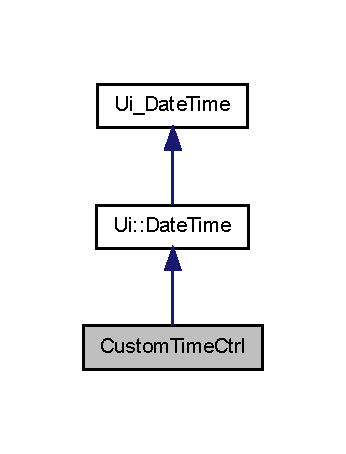
\includegraphics[width=166pt]{class_custom_time_ctrl__inherit__graph}
\end{center}
\end{figure}


Collaboration diagram for CustomTimeCtrl:\nopagebreak
\begin{figure}[H]
\begin{center}
\leavevmode
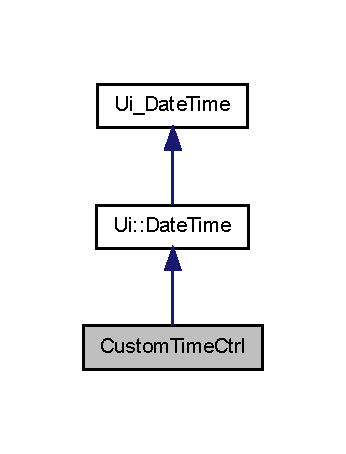
\includegraphics[width=166pt]{class_custom_time_ctrl__coll__graph}
\end{center}
\end{figure}
\subsection*{Public Slots}
\begin{DoxyCompactItemize}
\item 
void \hyperlink{class_custom_time_ctrl_ab385f1fff588560878db14f4ed1516cb}{adjustDateTime} (QModelIndex index, QVariant var)
\end{DoxyCompactItemize}
\subsection*{Signals}
\begin{DoxyCompactItemize}
\item 
void \hyperlink{class_custom_time_ctrl_aadc7a3337d1964c143c5d9da7bbc8f25}{isAuto} (bool bAuto)
\begin{DoxyCompactList}\small\item\em Is auto field. \item\end{DoxyCompactList}\item 
void \hyperlink{class_custom_time_ctrl_a7d9d68dbb0ad314e8e9e403b71398ac6}{isDateTime} (bool bDateTime, int row)
\begin{DoxyCompactList}\small\item\em Is auto field. \item\end{DoxyCompactList}\end{DoxyCompactItemize}
\subsection*{Public Member Functions}
\begin{DoxyCompactItemize}
\item 
\hyperlink{class_custom_time_ctrl_a2f6010d9bad7179ebb6067bc8c9c91f9}{CustomTimeCtrl} (QWidget $\ast$parent=0)
\item 
\hyperlink{class_custom_time_ctrl_a7d1b4fcf67ce5c636aed9943e1fc155d}{$\sim$CustomTimeCtrl} ()
\item 
void \hyperlink{class_custom_time_ctrl_ac9509ea1b691b78aa01aaa7b7311a7dc}{setDateTime} (const QDateTime \&datetime)
\begin{DoxyCompactList}\small\item\em Set DateTime. \item\end{DoxyCompactList}\item 
QDateTime \hyperlink{class_custom_time_ctrl_ac9aa79a88d07a399653990876740abba}{dateTime} ()
\item 
void \hyperlink{class_custom_time_ctrl_a00f254de688011ef033711d6d7873c2d}{setModelRow} (const int row)
\begin{DoxyCompactList}\small\item\em Set Model Row. \item\end{DoxyCompactList}\item 
void \hyperlink{class_custom_time_ctrl_ae25047958d9b33a8cef17fbb9d5aad39}{setIsDateTime} (const bool bDate, const bool bTime, const bool bCheck)
\begin{DoxyCompactList}\small\item\em Set Is Date Time. \item\end{DoxyCompactList}\item 
void \hyperlink{class_custom_time_ctrl_a630a9b3e818a5d0eb1fd45b812f1de80}{setIsUTC} (const bool bUTC)
\begin{DoxyCompactList}\small\item\em Set Is UTC. \item\end{DoxyCompactList}\item 
void \hyperlink{class_custom_time_ctrl_a6defd95e5d915f8b9b08a8b338283120}{setIsAuto} (const bool bAuto)
\begin{DoxyCompactList}\small\item\em Set Is Automatic. \item\end{DoxyCompactList}\item 
bool \hyperlink{class_custom_time_ctrl_a98ae9f9f769258df322419ce26ac7778}{getIsAuto} () const 
\begin{DoxyCompactList}\small\item\em Get Is Automatic. \item\end{DoxyCompactList}\item 
bool \hyperlink{class_custom_time_ctrl_a13d9d91b005bf7e9a585d5a49bba248c}{getIsUTC} () const 
\begin{DoxyCompactList}\small\item\em Get Is UTC. \item\end{DoxyCompactList}\item 
void \hyperlink{class_custom_time_ctrl_a87f05c08ece39484cbad24441f890d3c}{getIsDateTime} (bool \&bDate, bool \&bTime) const 
\begin{DoxyCompactList}\small\item\em Get Is DateTime. \item\end{DoxyCompactList}\item 
QCheckBox $\ast$ \hyperlink{class_custom_time_ctrl_a733c68c7cf18771530e05c55c0a2e3c0}{checkBox} ()
\begin{DoxyCompactList}\small\item\em Check Box. \item\end{DoxyCompactList}\item 
int \hyperlink{class_custom_time_ctrl_a3232a13b5a09af8d908162f5a3369f4c}{modelRow} () const 
\begin{DoxyCompactList}\small\item\em Model Row. \item\end{DoxyCompactList}\end{DoxyCompactItemize}
\subsection*{Protected Member Functions}
\begin{DoxyCompactItemize}
\item 
void \hyperlink{class_custom_time_ctrl_a32f81c6822f07b034d7291a4792bb936}{showEvent} (QShowEvent $\ast$event)
\begin{DoxyCompactList}\small\item\em Reimplementation from the method on the base class. \item\end{DoxyCompactList}\end{DoxyCompactItemize}
\subsection*{Properties}
\begin{DoxyCompactItemize}
\item 
QDateTime \hyperlink{class_custom_time_ctrl_ad091ad8a573db0fdf17366547aab5695}{dateTime}
\begin{DoxyCompactList}\small\item\em User Property exposed by this control (to be used by the QDataWidgetMapper and the Delegate) \item\end{DoxyCompactList}\end{DoxyCompactItemize}
\subsection*{Private Slots}
\begin{DoxyCompactItemize}
\item 
void \hyperlink{class_custom_time_ctrl_ae8a64e667cf921232d5d940ef7a3fce1}{setHasTime} (bool bTime)
\end{DoxyCompactItemize}
\subsection*{Private Member Functions}
\begin{DoxyCompactItemize}
\item 
void \hyperlink{class_custom_time_ctrl_ad1519295bb4900bc8c35a0885475140b}{setFormatInfo} ()
\begin{DoxyCompactList}\small\item\em Set Format Info. \item\end{DoxyCompactList}\item 
void \hyperlink{class_custom_time_ctrl_a049b8611ab15ec4ad46a93e7306ecc95}{showHasDateTime} ()
\begin{DoxyCompactList}\small\item\em Show HasDateTime. \item\end{DoxyCompactList}\end{DoxyCompactItemize}
\subsection*{Private Attributes}
\begin{DoxyCompactItemize}
\item 
bool \hyperlink{class_custom_time_ctrl_a24ca64a96066346b1d17414741143946}{m\_\-bCheck}
\begin{DoxyCompactList}\small\item\em Boolean flag to define if we wish to show the checkbox, allowing the optional datetime control. \item\end{DoxyCompactList}\item 
bool \hyperlink{class_custom_time_ctrl_ad400f22586d9744343b222469b7b044e}{m\_\-bDate}
\begin{DoxyCompactList}\small\item\em Boolean flag to define if the control exposes a date. \item\end{DoxyCompactList}\item 
bool \hyperlink{class_custom_time_ctrl_a0cf32d081f83b97e294f4170845a1439}{m\_\-bTime}
\begin{DoxyCompactList}\small\item\em Boolean flag to define if the control exposes a time. \item\end{DoxyCompactList}\item 
bool \hyperlink{class_custom_time_ctrl_a561551017a9fde5d281d23fa7c897903}{m\_\-bUTC}
\begin{DoxyCompactList}\small\item\em Boolean flag to define if the time object is in UTC. \item\end{DoxyCompactList}\item 
bool \hyperlink{class_custom_time_ctrl_a10051394dabcc7222ce57980c23a1554}{m\_\-bAuto}
\begin{DoxyCompactList}\small\item\em Boolean flag to define if this is an automatic datetime. \item\end{DoxyCompactList}\item 
int \hyperlink{class_custom_time_ctrl_aa0677acdf3557d4a7d63b6160f946d26}{m\_\-row}
\begin{DoxyCompactList}\small\item\em Integer to indicate the model row associated to this record. \item\end{DoxyCompactList}\end{DoxyCompactItemize}


\subsection{Detailed Description}
Custom Time Control class. This class decouples the DateTime Data Type in two separate widgets, for date and time; It also has some description properties to tells us if it is an automatic DateTime widget and if the time is UTC; 

\subsection{Constructor \& Destructor Documentation}
\hypertarget{class_custom_time_ctrl_a2f6010d9bad7179ebb6067bc8c9c91f9}{
\index{CustomTimeCtrl@{CustomTimeCtrl}!CustomTimeCtrl@{CustomTimeCtrl}}
\index{CustomTimeCtrl@{CustomTimeCtrl}!CustomTimeCtrl@{CustomTimeCtrl}}
\subsubsection[{CustomTimeCtrl}]{\setlength{\rightskip}{0pt plus 5cm}CustomTimeCtrl::CustomTimeCtrl (
\begin{DoxyParamCaption}
\item[{QWidget $\ast$}]{ parent = {\ttfamily 0}}
\end{DoxyParamCaption}
)}}
\label{class_custom_time_ctrl_a2f6010d9bad7179ebb6067bc8c9c91f9}


Here is the call graph for this function:\nopagebreak
\begin{figure}[H]
\begin{center}
\leavevmode
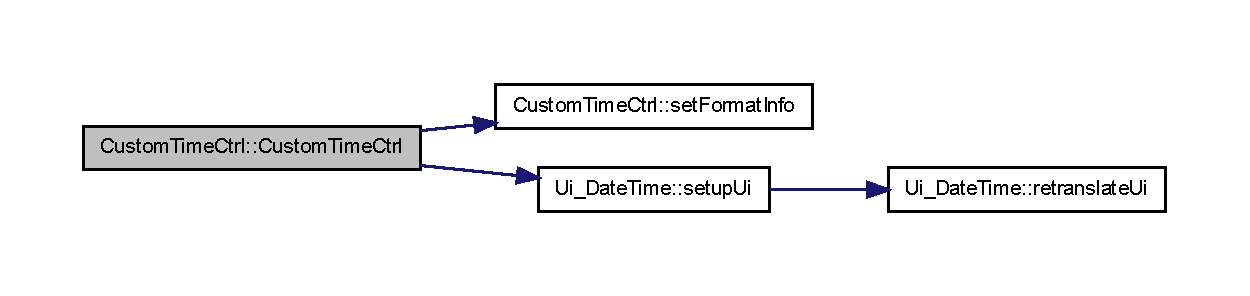
\includegraphics[width=400pt]{class_custom_time_ctrl_a2f6010d9bad7179ebb6067bc8c9c91f9_cgraph}
\end{center}
\end{figure}


\hypertarget{class_custom_time_ctrl_a7d1b4fcf67ce5c636aed9943e1fc155d}{
\index{CustomTimeCtrl@{CustomTimeCtrl}!$\sim$CustomTimeCtrl@{$\sim$CustomTimeCtrl}}
\index{$\sim$CustomTimeCtrl@{$\sim$CustomTimeCtrl}!CustomTimeCtrl@{CustomTimeCtrl}}
\subsubsection[{$\sim$CustomTimeCtrl}]{\setlength{\rightskip}{0pt plus 5cm}CustomTimeCtrl::$\sim$CustomTimeCtrl (
\begin{DoxyParamCaption}
{}
\end{DoxyParamCaption}
)}}
\label{class_custom_time_ctrl_a7d1b4fcf67ce5c636aed9943e1fc155d}


\subsection{Member Function Documentation}
\hypertarget{class_custom_time_ctrl_ab385f1fff588560878db14f4ed1516cb}{
\index{CustomTimeCtrl@{CustomTimeCtrl}!adjustDateTime@{adjustDateTime}}
\index{adjustDateTime@{adjustDateTime}!CustomTimeCtrl@{CustomTimeCtrl}}
\subsubsection[{adjustDateTime}]{\setlength{\rightskip}{0pt plus 5cm}void CustomTimeCtrl::adjustDateTime (
\begin{DoxyParamCaption}
\item[{QModelIndex}]{ index, }
\item[{QVariant}]{ var}
\end{DoxyParamCaption}
)\hspace{0.3cm}{\ttfamily  \mbox{[}slot\mbox{]}}}}
\label{class_custom_time_ctrl_ab385f1fff588560878db14f4ed1516cb}


Here is the call graph for this function:\nopagebreak
\begin{figure}[H]
\begin{center}
\leavevmode
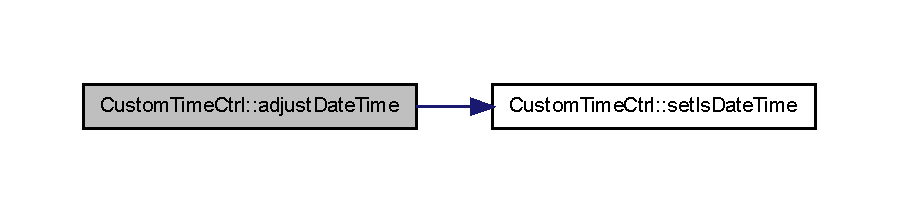
\includegraphics[width=400pt]{class_custom_time_ctrl_ab385f1fff588560878db14f4ed1516cb_cgraph}
\end{center}
\end{figure}


\hypertarget{class_custom_time_ctrl_a733c68c7cf18771530e05c55c0a2e3c0}{
\index{CustomTimeCtrl@{CustomTimeCtrl}!checkBox@{checkBox}}
\index{checkBox@{checkBox}!CustomTimeCtrl@{CustomTimeCtrl}}
\subsubsection[{checkBox}]{\setlength{\rightskip}{0pt plus 5cm}QCheckBox$\ast$ CustomTimeCtrl::checkBox (
\begin{DoxyParamCaption}
{}
\end{DoxyParamCaption}
)\hspace{0.3cm}{\ttfamily  \mbox{[}inline\mbox{]}}}}
\label{class_custom_time_ctrl_a733c68c7cf18771530e05c55c0a2e3c0}


Check Box. 

Convenience function that returns a pointer to the checkbox, that sets optional time. \hypertarget{class_custom_time_ctrl_ac9aa79a88d07a399653990876740abba}{
\index{CustomTimeCtrl@{CustomTimeCtrl}!dateTime@{dateTime}}
\index{dateTime@{dateTime}!CustomTimeCtrl@{CustomTimeCtrl}}
\subsubsection[{dateTime}]{\setlength{\rightskip}{0pt plus 5cm}QDateTime CustomTimeCtrl::dateTime (
\begin{DoxyParamCaption}
{}
\end{DoxyParamCaption}
)}}
\label{class_custom_time_ctrl_ac9aa79a88d07a399653990876740abba}
\hypertarget{class_custom_time_ctrl_a98ae9f9f769258df322419ce26ac7778}{
\index{CustomTimeCtrl@{CustomTimeCtrl}!getIsAuto@{getIsAuto}}
\index{getIsAuto@{getIsAuto}!CustomTimeCtrl@{CustomTimeCtrl}}
\subsubsection[{getIsAuto}]{\setlength{\rightskip}{0pt plus 5cm}bool CustomTimeCtrl::getIsAuto (
\begin{DoxyParamCaption}
{}
\end{DoxyParamCaption}
) const\hspace{0.3cm}{\ttfamily  \mbox{[}inline\mbox{]}}}}
\label{class_custom_time_ctrl_a98ae9f9f769258df322419ce26ac7778}


Get Is Automatic. 

Function to get if this is an automatic filled datetime (only current datetime is supported!) \hypertarget{class_custom_time_ctrl_a87f05c08ece39484cbad24441f890d3c}{
\index{CustomTimeCtrl@{CustomTimeCtrl}!getIsDateTime@{getIsDateTime}}
\index{getIsDateTime@{getIsDateTime}!CustomTimeCtrl@{CustomTimeCtrl}}
\subsubsection[{getIsDateTime}]{\setlength{\rightskip}{0pt plus 5cm}void CustomTimeCtrl::getIsDateTime (
\begin{DoxyParamCaption}
\item[{bool \&}]{ bDate, }
\item[{bool \&}]{ bTime}
\end{DoxyParamCaption}
) const\hspace{0.3cm}{\ttfamily  \mbox{[}inline\mbox{]}}}}
\label{class_custom_time_ctrl_a87f05c08ece39484cbad24441f890d3c}


Get Is DateTime. 

Function to get if this widget implements a date and/or a time; the result is stored in two boolean flags (for date and time); \begin{DoxyParagraph}{bdate Address of a boolean flag, where to store if this widget contains a date;}

\end{DoxyParagraph}
\begin{DoxyParagraph}{bTime Address of a boolean flag, where to store if this widget contains a time;}

\end{DoxyParagraph}
\hypertarget{class_custom_time_ctrl_a13d9d91b005bf7e9a585d5a49bba248c}{
\index{CustomTimeCtrl@{CustomTimeCtrl}!getIsUTC@{getIsUTC}}
\index{getIsUTC@{getIsUTC}!CustomTimeCtrl@{CustomTimeCtrl}}
\subsubsection[{getIsUTC}]{\setlength{\rightskip}{0pt plus 5cm}bool CustomTimeCtrl::getIsUTC (
\begin{DoxyParamCaption}
{}
\end{DoxyParamCaption}
) const\hspace{0.3cm}{\ttfamily  \mbox{[}inline\mbox{]}}}}
\label{class_custom_time_ctrl_a13d9d91b005bf7e9a585d5a49bba248c}


Get Is UTC. 

Function to get if the time represented in this widget is of type UTC; \hypertarget{class_custom_time_ctrl_aadc7a3337d1964c143c5d9da7bbc8f25}{
\index{CustomTimeCtrl@{CustomTimeCtrl}!isAuto@{isAuto}}
\index{isAuto@{isAuto}!CustomTimeCtrl@{CustomTimeCtrl}}
\subsubsection[{isAuto}]{\setlength{\rightskip}{0pt plus 5cm}void CustomTimeCtrl::isAuto (
\begin{DoxyParamCaption}
\item[{bool}]{ bAuto}
\end{DoxyParamCaption}
)\hspace{0.3cm}{\ttfamily  \mbox{[}signal\mbox{]}}}}
\label{class_custom_time_ctrl_aadc7a3337d1964c143c5d9da7bbc8f25}


Is auto field. 

Signal to indicate if this is an automatic field, that displays the current datetime. \begin{DoxyParagraph}{Auto boolean indicating if this is an auto field}

\end{DoxyParagraph}
\hypertarget{class_custom_time_ctrl_a7d9d68dbb0ad314e8e9e403b71398ac6}{
\index{CustomTimeCtrl@{CustomTimeCtrl}!isDateTime@{isDateTime}}
\index{isDateTime@{isDateTime}!CustomTimeCtrl@{CustomTimeCtrl}}
\subsubsection[{isDateTime}]{\setlength{\rightskip}{0pt plus 5cm}void CustomTimeCtrl::isDateTime (
\begin{DoxyParamCaption}
\item[{bool}]{ bDateTime, }
\item[{int}]{ row}
\end{DoxyParamCaption}
)\hspace{0.3cm}{\ttfamily  \mbox{[}signal\mbox{]}}}}
\label{class_custom_time_ctrl_a7d9d68dbb0ad314e8e9e403b71398ac6}


Is auto field. 

Signal to indicate if this is a datetime field. To ensure the synchronization with the model, we must also send the model row of the record associated with this widget, that has to be set beforehand. \begin{DoxyParagraph}{bDateTime boolean indicating if this is a datetime field}

\end{DoxyParagraph}
\begin{DoxyParagraph}{row integer with the model row for the (current) record;}

\end{DoxyParagraph}
\begin{DoxySeeAlso}{See also}
\hyperlink{class_custom_time_ctrl_a3232a13b5a09af8d908162f5a3369f4c}{modelRow()} 
\end{DoxySeeAlso}


Here is the caller graph for this function:\nopagebreak
\begin{figure}[H]
\begin{center}
\leavevmode
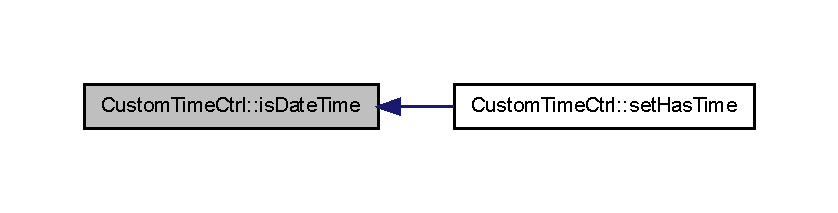
\includegraphics[width=400pt]{class_custom_time_ctrl_a7d9d68dbb0ad314e8e9e403b71398ac6_icgraph}
\end{center}
\end{figure}


\hypertarget{class_custom_time_ctrl_a3232a13b5a09af8d908162f5a3369f4c}{
\index{CustomTimeCtrl@{CustomTimeCtrl}!modelRow@{modelRow}}
\index{modelRow@{modelRow}!CustomTimeCtrl@{CustomTimeCtrl}}
\subsubsection[{modelRow}]{\setlength{\rightskip}{0pt plus 5cm}int CustomTimeCtrl::modelRow (
\begin{DoxyParamCaption}
{}
\end{DoxyParamCaption}
) const\hspace{0.3cm}{\ttfamily  \mbox{[}inline\mbox{]}}}}
\label{class_custom_time_ctrl_a3232a13b5a09af8d908162f5a3369f4c}


Model Row. 

Convenience function to return the model row; \hypertarget{class_custom_time_ctrl_ac9509ea1b691b78aa01aaa7b7311a7dc}{
\index{CustomTimeCtrl@{CustomTimeCtrl}!setDateTime@{setDateTime}}
\index{setDateTime@{setDateTime}!CustomTimeCtrl@{CustomTimeCtrl}}
\subsubsection[{setDateTime}]{\setlength{\rightskip}{0pt plus 5cm}void CustomTimeCtrl::setDateTime (
\begin{DoxyParamCaption}
\item[{const QDateTime \&}]{ datetime}
\end{DoxyParamCaption}
)}}
\label{class_custom_time_ctrl_ac9509ea1b691b78aa01aaa7b7311a7dc}


Set DateTime. 

Convenience function translate a datetime value in two different parts/widgets: date and time. \begin{DoxyParagraph}{datetime a datetime value.}

\end{DoxyParagraph}
\hypertarget{class_custom_time_ctrl_ad1519295bb4900bc8c35a0885475140b}{
\index{CustomTimeCtrl@{CustomTimeCtrl}!setFormatInfo@{setFormatInfo}}
\index{setFormatInfo@{setFormatInfo}!CustomTimeCtrl@{CustomTimeCtrl}}
\subsubsection[{setFormatInfo}]{\setlength{\rightskip}{0pt plus 5cm}void CustomTimeCtrl::setFormatInfo (
\begin{DoxyParamCaption}
{}
\end{DoxyParamCaption}
)\hspace{0.3cm}{\ttfamily  \mbox{[}private\mbox{]}}}}
\label{class_custom_time_ctrl_ad1519295bb4900bc8c35a0885475140b}


Set Format Info. 

Sets the labels with information about the current date/time format 

Here is the caller graph for this function:\nopagebreak
\begin{figure}[H]
\begin{center}
\leavevmode
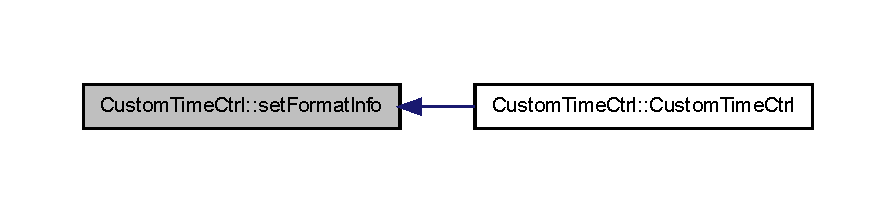
\includegraphics[width=400pt]{class_custom_time_ctrl_ad1519295bb4900bc8c35a0885475140b_icgraph}
\end{center}
\end{figure}


\hypertarget{class_custom_time_ctrl_ae8a64e667cf921232d5d940ef7a3fce1}{
\index{CustomTimeCtrl@{CustomTimeCtrl}!setHasTime@{setHasTime}}
\index{setHasTime@{setHasTime}!CustomTimeCtrl@{CustomTimeCtrl}}
\subsubsection[{setHasTime}]{\setlength{\rightskip}{0pt plus 5cm}void CustomTimeCtrl::setHasTime (
\begin{DoxyParamCaption}
\item[{bool}]{ bTime}
\end{DoxyParamCaption}
)\hspace{0.3cm}{\ttfamily  \mbox{[}private, slot\mbox{]}}}}
\label{class_custom_time_ctrl_ae8a64e667cf921232d5d940ef7a3fce1}


Here is the call graph for this function:\nopagebreak
\begin{figure}[H]
\begin{center}
\leavevmode
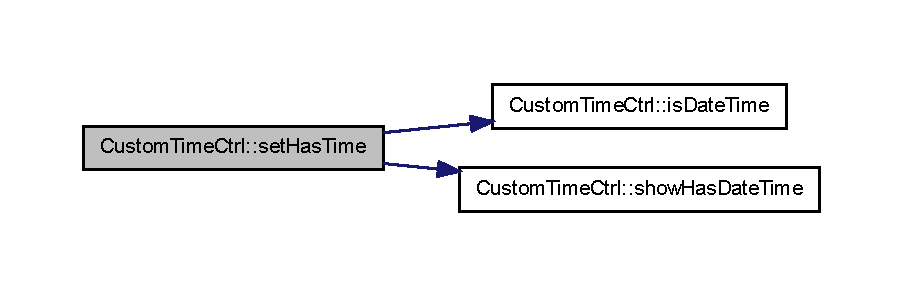
\includegraphics[width=400pt]{class_custom_time_ctrl_ae8a64e667cf921232d5d940ef7a3fce1_cgraph}
\end{center}
\end{figure}


\hypertarget{class_custom_time_ctrl_a6defd95e5d915f8b9b08a8b338283120}{
\index{CustomTimeCtrl@{CustomTimeCtrl}!setIsAuto@{setIsAuto}}
\index{setIsAuto@{setIsAuto}!CustomTimeCtrl@{CustomTimeCtrl}}
\subsubsection[{setIsAuto}]{\setlength{\rightskip}{0pt plus 5cm}void CustomTimeCtrl::setIsAuto (
\begin{DoxyParamCaption}
\item[{const bool}]{ bAuto}
\end{DoxyParamCaption}
)\hspace{0.3cm}{\ttfamily  \mbox{[}inline\mbox{]}}}}
\label{class_custom_time_ctrl_a6defd95e5d915f8b9b08a8b338283120}


Set Is Automatic. 

Function to set if this is an automatic filled datetime (only current datetime is supported!) \begin{DoxyParagraph}{bAuto boolean to flag if this time is an automatic datetime.}

\end{DoxyParagraph}
\hypertarget{class_custom_time_ctrl_ae25047958d9b33a8cef17fbb9d5aad39}{
\index{CustomTimeCtrl@{CustomTimeCtrl}!setIsDateTime@{setIsDateTime}}
\index{setIsDateTime@{setIsDateTime}!CustomTimeCtrl@{CustomTimeCtrl}}
\subsubsection[{setIsDateTime}]{\setlength{\rightskip}{0pt plus 5cm}void CustomTimeCtrl::setIsDateTime (
\begin{DoxyParamCaption}
\item[{const bool}]{ bDate, }
\item[{const bool}]{ bTime, }
\item[{const bool}]{ bCheck}
\end{DoxyParamCaption}
)}}
\label{class_custom_time_ctrl_ae25047958d9b33a8cef17fbb9d5aad39}


Set Is Date Time. 

Function to set if this widget implements a date and/or a time; \begin{DoxyParagraph}{bDate boolean to flag if this widget implements a date.}

\end{DoxyParagraph}
\begin{DoxyParagraph}{bTime boolean to flag if this widget implements a time.}

\end{DoxyParagraph}
\begin{DoxyParagraph}{bCheck boolean to flag if this widget has an optional time part.}

\end{DoxyParagraph}


Here is the caller graph for this function:\nopagebreak
\begin{figure}[H]
\begin{center}
\leavevmode
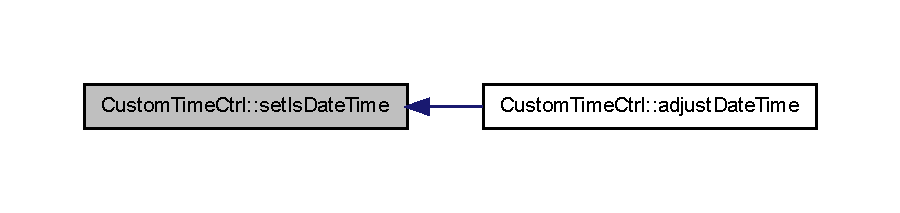
\includegraphics[width=400pt]{class_custom_time_ctrl_ae25047958d9b33a8cef17fbb9d5aad39_icgraph}
\end{center}
\end{figure}


\hypertarget{class_custom_time_ctrl_a630a9b3e818a5d0eb1fd45b812f1de80}{
\index{CustomTimeCtrl@{CustomTimeCtrl}!setIsUTC@{setIsUTC}}
\index{setIsUTC@{setIsUTC}!CustomTimeCtrl@{CustomTimeCtrl}}
\subsubsection[{setIsUTC}]{\setlength{\rightskip}{0pt plus 5cm}void CustomTimeCtrl::setIsUTC (
\begin{DoxyParamCaption}
\item[{const bool}]{ bUTC}
\end{DoxyParamCaption}
)\hspace{0.3cm}{\ttfamily  \mbox{[}inline\mbox{]}}}}
\label{class_custom_time_ctrl_a630a9b3e818a5d0eb1fd45b812f1de80}


Set Is UTC. 

Function to set if the time represented in this widget is of type UTC; \begin{DoxyParagraph}{bUTC boolean to flag if this time is UTC.}

\end{DoxyParagraph}
\hypertarget{class_custom_time_ctrl_a00f254de688011ef033711d6d7873c2d}{
\index{CustomTimeCtrl@{CustomTimeCtrl}!setModelRow@{setModelRow}}
\index{setModelRow@{setModelRow}!CustomTimeCtrl@{CustomTimeCtrl}}
\subsubsection[{setModelRow}]{\setlength{\rightskip}{0pt plus 5cm}void CustomTimeCtrl::setModelRow (
\begin{DoxyParamCaption}
\item[{const int}]{ row}
\end{DoxyParamCaption}
)\hspace{0.3cm}{\ttfamily  \mbox{[}inline\mbox{]}}}}
\label{class_custom_time_ctrl_a00f254de688011ef033711d6d7873c2d}


Set Model Row. 

Function to set the model row that corresponds to the record currently displayed on this widget. \begin{DoxyParagraph}{row model row, as integer.}

\end{DoxyParagraph}
\hypertarget{class_custom_time_ctrl_a32f81c6822f07b034d7291a4792bb936}{
\index{CustomTimeCtrl@{CustomTimeCtrl}!showEvent@{showEvent}}
\index{showEvent@{showEvent}!CustomTimeCtrl@{CustomTimeCtrl}}
\subsubsection[{showEvent}]{\setlength{\rightskip}{0pt plus 5cm}void CustomTimeCtrl::showEvent (
\begin{DoxyParamCaption}
\item[{QShowEvent $\ast$}]{ event}
\end{DoxyParamCaption}
)\hspace{0.3cm}{\ttfamily  \mbox{[}protected\mbox{]}}}}
\label{class_custom_time_ctrl_a32f81c6822f07b034d7291a4792bb936}


Reimplementation from the method on the base class. 

Method call on the show event; \begin{DoxyParagraph}{event an event}

\end{DoxyParagraph}


Here is the call graph for this function:\nopagebreak
\begin{figure}[H]
\begin{center}
\leavevmode
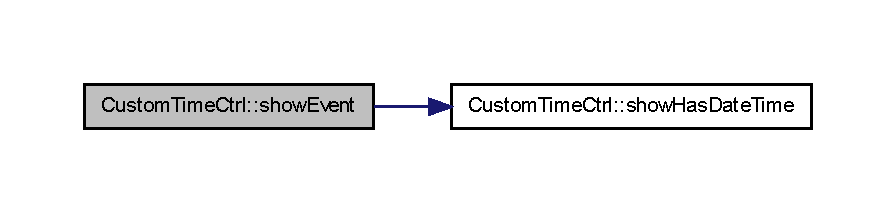
\includegraphics[width=400pt]{class_custom_time_ctrl_a32f81c6822f07b034d7291a4792bb936_cgraph}
\end{center}
\end{figure}


\hypertarget{class_custom_time_ctrl_a049b8611ab15ec4ad46a93e7306ecc95}{
\index{CustomTimeCtrl@{CustomTimeCtrl}!showHasDateTime@{showHasDateTime}}
\index{showHasDateTime@{showHasDateTime}!CustomTimeCtrl@{CustomTimeCtrl}}
\subsubsection[{showHasDateTime}]{\setlength{\rightskip}{0pt plus 5cm}void CustomTimeCtrl::showHasDateTime (
\begin{DoxyParamCaption}
{}
\end{DoxyParamCaption}
)\hspace{0.3cm}{\ttfamily  \mbox{[}private\mbox{]}}}}
\label{class_custom_time_ctrl_a049b8611ab15ec4ad46a93e7306ecc95}


Show HasDateTime. 

This method displays the widget with all the available options (checkbox that allows switching on/off the time). 

Here is the caller graph for this function:\nopagebreak
\begin{figure}[H]
\begin{center}
\leavevmode
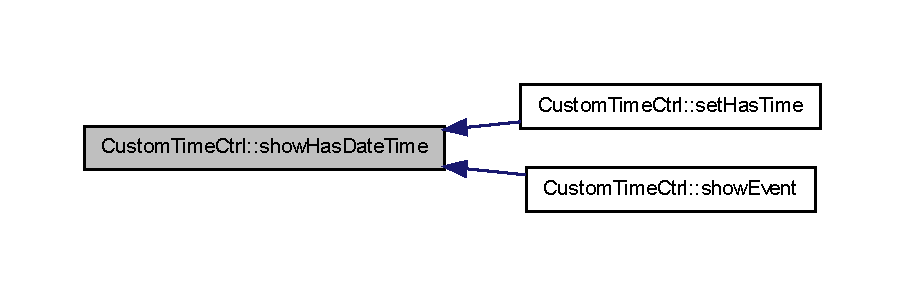
\includegraphics[width=400pt]{class_custom_time_ctrl_a049b8611ab15ec4ad46a93e7306ecc95_icgraph}
\end{center}
\end{figure}




\subsection{Member Data Documentation}
\hypertarget{class_custom_time_ctrl_a10051394dabcc7222ce57980c23a1554}{
\index{CustomTimeCtrl@{CustomTimeCtrl}!m\_\-bAuto@{m\_\-bAuto}}
\index{m\_\-bAuto@{m\_\-bAuto}!CustomTimeCtrl@{CustomTimeCtrl}}
\subsubsection[{m\_\-bAuto}]{\setlength{\rightskip}{0pt plus 5cm}bool {\bf CustomTimeCtrl::m\_\-bAuto}\hspace{0.3cm}{\ttfamily  \mbox{[}private\mbox{]}}}}
\label{class_custom_time_ctrl_a10051394dabcc7222ce57980c23a1554}


Boolean flag to define if this is an automatic datetime. 

\hypertarget{class_custom_time_ctrl_a24ca64a96066346b1d17414741143946}{
\index{CustomTimeCtrl@{CustomTimeCtrl}!m\_\-bCheck@{m\_\-bCheck}}
\index{m\_\-bCheck@{m\_\-bCheck}!CustomTimeCtrl@{CustomTimeCtrl}}
\subsubsection[{m\_\-bCheck}]{\setlength{\rightskip}{0pt plus 5cm}bool {\bf CustomTimeCtrl::m\_\-bCheck}\hspace{0.3cm}{\ttfamily  \mbox{[}private\mbox{]}}}}
\label{class_custom_time_ctrl_a24ca64a96066346b1d17414741143946}


Boolean flag to define if we wish to show the checkbox, allowing the optional datetime control. 

\hypertarget{class_custom_time_ctrl_ad400f22586d9744343b222469b7b044e}{
\index{CustomTimeCtrl@{CustomTimeCtrl}!m\_\-bDate@{m\_\-bDate}}
\index{m\_\-bDate@{m\_\-bDate}!CustomTimeCtrl@{CustomTimeCtrl}}
\subsubsection[{m\_\-bDate}]{\setlength{\rightskip}{0pt plus 5cm}bool {\bf CustomTimeCtrl::m\_\-bDate}\hspace{0.3cm}{\ttfamily  \mbox{[}private\mbox{]}}}}
\label{class_custom_time_ctrl_ad400f22586d9744343b222469b7b044e}


Boolean flag to define if the control exposes a date. 

\hypertarget{class_custom_time_ctrl_a0cf32d081f83b97e294f4170845a1439}{
\index{CustomTimeCtrl@{CustomTimeCtrl}!m\_\-bTime@{m\_\-bTime}}
\index{m\_\-bTime@{m\_\-bTime}!CustomTimeCtrl@{CustomTimeCtrl}}
\subsubsection[{m\_\-bTime}]{\setlength{\rightskip}{0pt plus 5cm}bool {\bf CustomTimeCtrl::m\_\-bTime}\hspace{0.3cm}{\ttfamily  \mbox{[}private\mbox{]}}}}
\label{class_custom_time_ctrl_a0cf32d081f83b97e294f4170845a1439}


Boolean flag to define if the control exposes a time. 

\hypertarget{class_custom_time_ctrl_a561551017a9fde5d281d23fa7c897903}{
\index{CustomTimeCtrl@{CustomTimeCtrl}!m\_\-bUTC@{m\_\-bUTC}}
\index{m\_\-bUTC@{m\_\-bUTC}!CustomTimeCtrl@{CustomTimeCtrl}}
\subsubsection[{m\_\-bUTC}]{\setlength{\rightskip}{0pt plus 5cm}bool {\bf CustomTimeCtrl::m\_\-bUTC}\hspace{0.3cm}{\ttfamily  \mbox{[}private\mbox{]}}}}
\label{class_custom_time_ctrl_a561551017a9fde5d281d23fa7c897903}


Boolean flag to define if the time object is in UTC. 

\hypertarget{class_custom_time_ctrl_aa0677acdf3557d4a7d63b6160f946d26}{
\index{CustomTimeCtrl@{CustomTimeCtrl}!m\_\-row@{m\_\-row}}
\index{m\_\-row@{m\_\-row}!CustomTimeCtrl@{CustomTimeCtrl}}
\subsubsection[{m\_\-row}]{\setlength{\rightskip}{0pt plus 5cm}int {\bf CustomTimeCtrl::m\_\-row}\hspace{0.3cm}{\ttfamily  \mbox{[}private\mbox{]}}}}
\label{class_custom_time_ctrl_aa0677acdf3557d4a7d63b6160f946d26}


Integer to indicate the model row associated to this record. 



\subsection{Property Documentation}
\hypertarget{class_custom_time_ctrl_ad091ad8a573db0fdf17366547aab5695}{
\index{CustomTimeCtrl@{CustomTimeCtrl}!dateTime@{dateTime}}
\index{dateTime@{dateTime}!CustomTimeCtrl@{CustomTimeCtrl}}
\subsubsection[{dateTime}]{\setlength{\rightskip}{0pt plus 5cm}QDateTime CustomTimeCtrl::dateTime\hspace{0.3cm}{\ttfamily  \mbox{[}read, write\mbox{]}}}}
\label{class_custom_time_ctrl_ad091ad8a573db0fdf17366547aab5695}


User Property exposed by this control (to be used by the QDataWidgetMapper and the Delegate) 



The documentation for this class was generated from the following files:\begin{DoxyCompactItemize}
\item 
CustomTimeCtrl/\hyperlink{customtimectrl_8h}{customtimectrl.h}\item 
CustomTimeCtrl/\hyperlink{customtimectrl_8cpp}{customtimectrl.cpp}\item 
CustomTimeCtrl/GeneratedFiles/Debug/\hyperlink{_debug_2moc__customtimectrl_8cpp}{moc\_\-customtimectrl.cpp}\item 
CustomTimeCtrl/GeneratedFiles/Release/\hyperlink{_release_2moc__customtimectrl_8cpp}{moc\_\-customtimectrl.cpp}\end{DoxyCompactItemize}

\hypertarget{class_custom_time_ctrl_plugin}{
\section{CustomTimeCtrlPlugin Class Reference}
\label{class_custom_time_ctrl_plugin}\index{CustomTimeCtrlPlugin@{CustomTimeCtrlPlugin}}
}


Plugin Class.  




{\ttfamily \#include $<$customtimectrlplugin.h$>$}

\subsection*{Public Member Functions}
\begin{DoxyCompactItemize}
\item 
\hyperlink{class_custom_time_ctrl_plugin_abe7cd3182b486842f7dc7f13a5b4c087}{CustomTimeCtrlPlugin} (QObject $\ast$parent=0)
\item 
bool \hyperlink{class_custom_time_ctrl_plugin_ac3f03f248edec95fb4d8e50596adbcbb}{isContainer} () const 
\item 
bool \hyperlink{class_custom_time_ctrl_plugin_a2064723849d9484c5c84aa7ad901274d}{isInitialized} () const 
\item 
QIcon \hyperlink{class_custom_time_ctrl_plugin_ae0dea4f3f0275ab82f97af2f1cd09e9a}{icon} () const 
\begin{DoxyCompactList}\small\item\em Icon for this plugin;. \item\end{DoxyCompactList}\item 
QString \hyperlink{class_custom_time_ctrl_plugin_a67b84de1996b4765eaaf3bb19ae79a1c}{domXml} () const 
\item 
QString \hyperlink{class_custom_time_ctrl_plugin_a3d53c6dcaf283efd9329d8b248c7d403}{group} () const 
\begin{DoxyCompactList}\small\item\em Group for this plugin, in the Designer;. \item\end{DoxyCompactList}\item 
QString \hyperlink{class_custom_time_ctrl_plugin_a873b662cfddffa85ad084a89091cd587}{includeFile} () const 
\begin{DoxyCompactList}\small\item\em Include file for the plugin;. \item\end{DoxyCompactList}\item 
QString \hyperlink{class_custom_time_ctrl_plugin_a4b34d287a8c4491229ee6e8bf6e9575a}{name} () const 
\begin{DoxyCompactList}\small\item\em Plugin name;. \item\end{DoxyCompactList}\item 
QString \hyperlink{class_custom_time_ctrl_plugin_a105774fa13b7f9df40f497aa582722df}{toolTip} () const 
\begin{DoxyCompactList}\small\item\em Plugin tooltip;. \item\end{DoxyCompactList}\item 
QString \hyperlink{class_custom_time_ctrl_plugin_aa37c7e879b0e8b6eb4e0e0ec32331dd6}{whatsThis} () const 
\begin{DoxyCompactList}\small\item\em Plugin whatsThis;. \item\end{DoxyCompactList}\item 
QWidget $\ast$ \hyperlink{class_custom_time_ctrl_plugin_aaf1a4b91242dab7caaa3194a54fa7cd3}{createWidget} (QWidget $\ast$parent)
\begin{DoxyCompactList}\small\item\em Method that instantiates the customtimectrl class (and therefore the control);. \item\end{DoxyCompactList}\item 
void \hyperlink{class_custom_time_ctrl_plugin_a71b6bce209cc6beff5ab3b6c12bcf1ab}{initialize} (QDesignerFormEditorInterface $\ast$core)
\end{DoxyCompactItemize}
\subsection*{Private Attributes}
\begin{DoxyCompactItemize}
\item 
bool \hyperlink{class_custom_time_ctrl_plugin_a7c04fd49d79c4936052dd81dcb9a2787}{initialized}
\end{DoxyCompactItemize}


\subsection{Detailed Description}
Plugin Class. This is the class exposed as a plugin; it is ihneritated from QDesignerCustomWidgetInterface, which is an custom class for Qt designer plugins. 

\subsection{Constructor \& Destructor Documentation}
\hypertarget{class_custom_time_ctrl_plugin_abe7cd3182b486842f7dc7f13a5b4c087}{
\index{CustomTimeCtrlPlugin@{CustomTimeCtrlPlugin}!CustomTimeCtrlPlugin@{CustomTimeCtrlPlugin}}
\index{CustomTimeCtrlPlugin@{CustomTimeCtrlPlugin}!CustomTimeCtrlPlugin@{CustomTimeCtrlPlugin}}
\subsubsection[{CustomTimeCtrlPlugin}]{\setlength{\rightskip}{0pt plus 5cm}CustomTimeCtrlPlugin::CustomTimeCtrlPlugin (
\begin{DoxyParamCaption}
\item[{QObject $\ast$}]{ parent = {\ttfamily 0}}
\end{DoxyParamCaption}
)}}
\label{class_custom_time_ctrl_plugin_abe7cd3182b486842f7dc7f13a5b4c087}


\subsection{Member Function Documentation}
\hypertarget{class_custom_time_ctrl_plugin_aaf1a4b91242dab7caaa3194a54fa7cd3}{
\index{CustomTimeCtrlPlugin@{CustomTimeCtrlPlugin}!createWidget@{createWidget}}
\index{createWidget@{createWidget}!CustomTimeCtrlPlugin@{CustomTimeCtrlPlugin}}
\subsubsection[{createWidget}]{\setlength{\rightskip}{0pt plus 5cm}QWidget $\ast$ CustomTimeCtrlPlugin::createWidget (
\begin{DoxyParamCaption}
\item[{QWidget $\ast$}]{ parent}
\end{DoxyParamCaption}
)}}
\label{class_custom_time_ctrl_plugin_aaf1a4b91242dab7caaa3194a54fa7cd3}


Method that instantiates the customtimectrl class (and therefore the control);. 

\hypertarget{class_custom_time_ctrl_plugin_a67b84de1996b4765eaaf3bb19ae79a1c}{
\index{CustomTimeCtrlPlugin@{CustomTimeCtrlPlugin}!domXml@{domXml}}
\index{domXml@{domXml}!CustomTimeCtrlPlugin@{CustomTimeCtrlPlugin}}
\subsubsection[{domXml}]{\setlength{\rightskip}{0pt plus 5cm}QString CustomTimeCtrlPlugin::domXml (
\begin{DoxyParamCaption}
{}
\end{DoxyParamCaption}
) const}}
\label{class_custom_time_ctrl_plugin_a67b84de1996b4765eaaf3bb19ae79a1c}
\hypertarget{class_custom_time_ctrl_plugin_a3d53c6dcaf283efd9329d8b248c7d403}{
\index{CustomTimeCtrlPlugin@{CustomTimeCtrlPlugin}!group@{group}}
\index{group@{group}!CustomTimeCtrlPlugin@{CustomTimeCtrlPlugin}}
\subsubsection[{group}]{\setlength{\rightskip}{0pt plus 5cm}QString CustomTimeCtrlPlugin::group (
\begin{DoxyParamCaption}
{}
\end{DoxyParamCaption}
) const}}
\label{class_custom_time_ctrl_plugin_a3d53c6dcaf283efd9329d8b248c7d403}


Group for this plugin, in the Designer;. 

\hypertarget{class_custom_time_ctrl_plugin_ae0dea4f3f0275ab82f97af2f1cd09e9a}{
\index{CustomTimeCtrlPlugin@{CustomTimeCtrlPlugin}!icon@{icon}}
\index{icon@{icon}!CustomTimeCtrlPlugin@{CustomTimeCtrlPlugin}}
\subsubsection[{icon}]{\setlength{\rightskip}{0pt plus 5cm}QIcon CustomTimeCtrlPlugin::icon (
\begin{DoxyParamCaption}
{}
\end{DoxyParamCaption}
) const}}
\label{class_custom_time_ctrl_plugin_ae0dea4f3f0275ab82f97af2f1cd09e9a}


Icon for this plugin;. 

\hypertarget{class_custom_time_ctrl_plugin_a873b662cfddffa85ad084a89091cd587}{
\index{CustomTimeCtrlPlugin@{CustomTimeCtrlPlugin}!includeFile@{includeFile}}
\index{includeFile@{includeFile}!CustomTimeCtrlPlugin@{CustomTimeCtrlPlugin}}
\subsubsection[{includeFile}]{\setlength{\rightskip}{0pt plus 5cm}QString CustomTimeCtrlPlugin::includeFile (
\begin{DoxyParamCaption}
{}
\end{DoxyParamCaption}
) const}}
\label{class_custom_time_ctrl_plugin_a873b662cfddffa85ad084a89091cd587}


Include file for the plugin;. 

\hypertarget{class_custom_time_ctrl_plugin_a71b6bce209cc6beff5ab3b6c12bcf1ab}{
\index{CustomTimeCtrlPlugin@{CustomTimeCtrlPlugin}!initialize@{initialize}}
\index{initialize@{initialize}!CustomTimeCtrlPlugin@{CustomTimeCtrlPlugin}}
\subsubsection[{initialize}]{\setlength{\rightskip}{0pt plus 5cm}void CustomTimeCtrlPlugin::initialize (
\begin{DoxyParamCaption}
\item[{QDesignerFormEditorInterface $\ast$}]{ core}
\end{DoxyParamCaption}
)}}
\label{class_custom_time_ctrl_plugin_a71b6bce209cc6beff5ab3b6c12bcf1ab}
\hypertarget{class_custom_time_ctrl_plugin_ac3f03f248edec95fb4d8e50596adbcbb}{
\index{CustomTimeCtrlPlugin@{CustomTimeCtrlPlugin}!isContainer@{isContainer}}
\index{isContainer@{isContainer}!CustomTimeCtrlPlugin@{CustomTimeCtrlPlugin}}
\subsubsection[{isContainer}]{\setlength{\rightskip}{0pt plus 5cm}bool CustomTimeCtrlPlugin::isContainer (
\begin{DoxyParamCaption}
{}
\end{DoxyParamCaption}
) const}}
\label{class_custom_time_ctrl_plugin_ac3f03f248edec95fb4d8e50596adbcbb}
\hypertarget{class_custom_time_ctrl_plugin_a2064723849d9484c5c84aa7ad901274d}{
\index{CustomTimeCtrlPlugin@{CustomTimeCtrlPlugin}!isInitialized@{isInitialized}}
\index{isInitialized@{isInitialized}!CustomTimeCtrlPlugin@{CustomTimeCtrlPlugin}}
\subsubsection[{isInitialized}]{\setlength{\rightskip}{0pt plus 5cm}bool CustomTimeCtrlPlugin::isInitialized (
\begin{DoxyParamCaption}
{}
\end{DoxyParamCaption}
) const}}
\label{class_custom_time_ctrl_plugin_a2064723849d9484c5c84aa7ad901274d}
\hypertarget{class_custom_time_ctrl_plugin_a4b34d287a8c4491229ee6e8bf6e9575a}{
\index{CustomTimeCtrlPlugin@{CustomTimeCtrlPlugin}!name@{name}}
\index{name@{name}!CustomTimeCtrlPlugin@{CustomTimeCtrlPlugin}}
\subsubsection[{name}]{\setlength{\rightskip}{0pt plus 5cm}QString CustomTimeCtrlPlugin::name (
\begin{DoxyParamCaption}
{}
\end{DoxyParamCaption}
) const}}
\label{class_custom_time_ctrl_plugin_a4b34d287a8c4491229ee6e8bf6e9575a}


Plugin name;. 

\hypertarget{class_custom_time_ctrl_plugin_a105774fa13b7f9df40f497aa582722df}{
\index{CustomTimeCtrlPlugin@{CustomTimeCtrlPlugin}!toolTip@{toolTip}}
\index{toolTip@{toolTip}!CustomTimeCtrlPlugin@{CustomTimeCtrlPlugin}}
\subsubsection[{toolTip}]{\setlength{\rightskip}{0pt plus 5cm}QString CustomTimeCtrlPlugin::toolTip (
\begin{DoxyParamCaption}
{}
\end{DoxyParamCaption}
) const}}
\label{class_custom_time_ctrl_plugin_a105774fa13b7f9df40f497aa582722df}


Plugin tooltip;. 

\hypertarget{class_custom_time_ctrl_plugin_aa37c7e879b0e8b6eb4e0e0ec32331dd6}{
\index{CustomTimeCtrlPlugin@{CustomTimeCtrlPlugin}!whatsThis@{whatsThis}}
\index{whatsThis@{whatsThis}!CustomTimeCtrlPlugin@{CustomTimeCtrlPlugin}}
\subsubsection[{whatsThis}]{\setlength{\rightskip}{0pt plus 5cm}QString CustomTimeCtrlPlugin::whatsThis (
\begin{DoxyParamCaption}
{}
\end{DoxyParamCaption}
) const}}
\label{class_custom_time_ctrl_plugin_aa37c7e879b0e8b6eb4e0e0ec32331dd6}


Plugin whatsThis;. 



\subsection{Member Data Documentation}
\hypertarget{class_custom_time_ctrl_plugin_a7c04fd49d79c4936052dd81dcb9a2787}{
\index{CustomTimeCtrlPlugin@{CustomTimeCtrlPlugin}!initialized@{initialized}}
\index{initialized@{initialized}!CustomTimeCtrlPlugin@{CustomTimeCtrlPlugin}}
\subsubsection[{initialized}]{\setlength{\rightskip}{0pt plus 5cm}bool {\bf CustomTimeCtrlPlugin::initialized}\hspace{0.3cm}{\ttfamily  \mbox{[}private\mbox{]}}}}
\label{class_custom_time_ctrl_plugin_a7c04fd49d79c4936052dd81dcb9a2787}


The documentation for this class was generated from the following files:\begin{DoxyCompactItemize}
\item 
CustomTimeCtrl/\hyperlink{customtimectrlplugin_8h}{customtimectrlplugin.h}\item 
CustomTimeCtrl/\hyperlink{customtimectrlplugin_8cpp}{customtimectrlplugin.cpp}\end{DoxyCompactItemize}

\hypertarget{class_ui_1_1_date_time}{
\section{Ui::DateTime Class Reference}
\label{class_ui_1_1_date_time}\index{Ui::DateTime@{Ui::DateTime}}
}


{\ttfamily \#include $<$ui\_\-datetime.h$>$}



Inheritance diagram for Ui::DateTime:\nopagebreak
\begin{figure}[H]
\begin{center}
\leavevmode
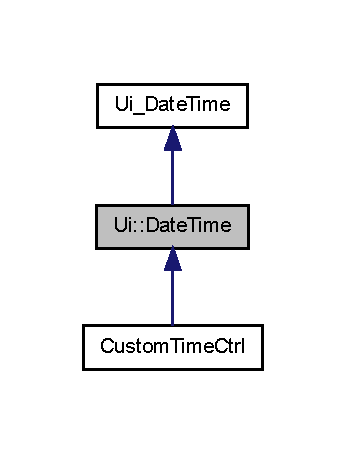
\includegraphics[width=166pt]{class_ui_1_1_date_time__inherit__graph}
\end{center}
\end{figure}


Collaboration diagram for Ui::DateTime:\nopagebreak
\begin{figure}[H]
\begin{center}
\leavevmode
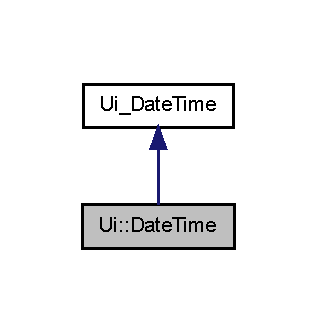
\includegraphics[width=152pt]{class_ui_1_1_date_time__coll__graph}
\end{center}
\end{figure}


The documentation for this class was generated from the following file:\begin{DoxyCompactItemize}
\item 
CustomTimeCtrl/GeneratedFiles/\hyperlink{ui__datetime_8h}{ui\_\-datetime.h}\end{DoxyCompactItemize}

\hypertarget{class_ui___date_time}{
\section{Ui\_\-DateTime Class Reference}
\label{class_ui___date_time}\index{Ui\_\-DateTime@{Ui\_\-DateTime}}
}


{\ttfamily \#include $<$ui\_\-datetime.h$>$}



Inheritance diagram for Ui\_\-DateTime:\nopagebreak
\begin{figure}[H]
\begin{center}
\leavevmode
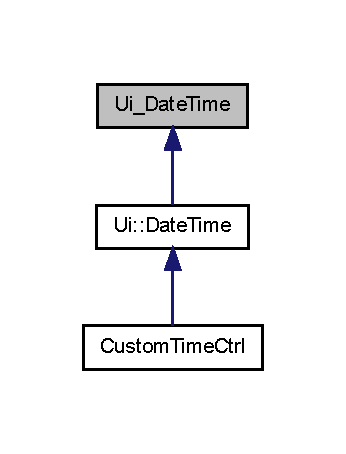
\includegraphics[width=166pt]{class_ui___date_time__inherit__graph}
\end{center}
\end{figure}
\subsection*{Public Member Functions}
\begin{DoxyCompactItemize}
\item 
void \hyperlink{class_ui___date_time_aec460e980f671b301914cde3e3802143}{setupUi} (QWidget $\ast$DateTime)
\item 
void \hyperlink{class_ui___date_time_aa8b20acb5b090ebf9e2492f0ec58689f}{retranslateUi} (QWidget $\ast$DateTime)
\end{DoxyCompactItemize}
\subsection*{Public Attributes}
\begin{DoxyCompactItemize}
\item 
QVBoxLayout $\ast$ \hyperlink{class_ui___date_time_a5b1cbbfbf53e56fae7a1d7010cd6dd78}{verticalLayout}
\item 
QHBoxLayout $\ast$ \hyperlink{class_ui___date_time_a4a83e6da2cb4777c714707d0ec9ef071}{horizontalLayout\_\-2}
\item 
QGroupBox $\ast$ \hyperlink{class_ui___date_time_aa589c9b11f049e55441921472edf5edb}{groupDate}
\item 
QGridLayout $\ast$ \hyperlink{class_ui___date_time_afd7d89b895d622f67653fc453dc781a7}{gridLayout}
\item 
QLabel $\ast$ \hyperlink{class_ui___date_time_a2c9c40ac284a6523d361201e4c0c2ec7}{lbDate}
\item 
QDateEdit $\ast$ \hyperlink{class_ui___date_time_ac05a6b58da81b4d73730ab4deffc37d7}{dateEdit}
\item 
QLabel $\ast$ \hyperlink{class_ui___date_time_ae2e82ce0d9b527827658c605e4f814e7}{lbDateFormat}
\item 
QGroupBox $\ast$ \hyperlink{class_ui___date_time_a0228c72e4210b7e2325f003f7b0525bd}{groupTime}
\item 
QGridLayout $\ast$ \hyperlink{class_ui___date_time_a5e283d401d2a14332b5c057dca4b5191}{gridLayout\_\-2}
\item 
QLabel $\ast$ \hyperlink{class_ui___date_time_a3a3c6501192cd0e3d6586310689bcd3f}{lbTime}
\item 
QTimeEdit $\ast$ \hyperlink{class_ui___date_time_a37289c6e591cee258708a9736b503415}{timeEdit}
\item 
QLabel $\ast$ \hyperlink{class_ui___date_time_a8701c245df77db5561ea1c0964c20a8f}{lbTimeFormat}
\item 
QGroupBox $\ast$ \hyperlink{class_ui___date_time_ae9887b3a8b4e56cf1cac0d542819c98d}{groupHasTime}
\item 
QHBoxLayout $\ast$ \hyperlink{class_ui___date_time_a2643fceafcdce6541af710a79f579301}{horizontalLayout}
\item 
QCheckBox $\ast$ \hyperlink{class_ui___date_time_acd3af509eccfb3a359c9a76ea8dfa2d4}{checkTime}
\end{DoxyCompactItemize}


\subsection{Member Function Documentation}
\hypertarget{class_ui___date_time_aa8b20acb5b090ebf9e2492f0ec58689f}{
\index{Ui\_\-DateTime@{Ui\_\-DateTime}!retranslateUi@{retranslateUi}}
\index{retranslateUi@{retranslateUi}!Ui_DateTime@{Ui\_\-DateTime}}
\subsubsection[{retranslateUi}]{\setlength{\rightskip}{0pt plus 5cm}void Ui\_\-DateTime::retranslateUi (
\begin{DoxyParamCaption}
\item[{QWidget $\ast$}]{ DateTime}
\end{DoxyParamCaption}
)\hspace{0.3cm}{\ttfamily  \mbox{[}inline\mbox{]}}}}
\label{class_ui___date_time_aa8b20acb5b090ebf9e2492f0ec58689f}


Here is the caller graph for this function:\nopagebreak
\begin{figure}[H]
\begin{center}
\leavevmode
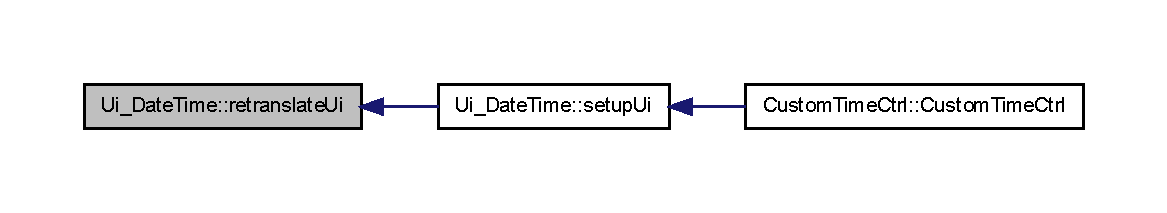
\includegraphics[width=400pt]{class_ui___date_time_aa8b20acb5b090ebf9e2492f0ec58689f_icgraph}
\end{center}
\end{figure}


\hypertarget{class_ui___date_time_aec460e980f671b301914cde3e3802143}{
\index{Ui\_\-DateTime@{Ui\_\-DateTime}!setupUi@{setupUi}}
\index{setupUi@{setupUi}!Ui_DateTime@{Ui\_\-DateTime}}
\subsubsection[{setupUi}]{\setlength{\rightskip}{0pt plus 5cm}void Ui\_\-DateTime::setupUi (
\begin{DoxyParamCaption}
\item[{QWidget $\ast$}]{ DateTime}
\end{DoxyParamCaption}
)\hspace{0.3cm}{\ttfamily  \mbox{[}inline\mbox{]}}}}
\label{class_ui___date_time_aec460e980f671b301914cde3e3802143}


Here is the call graph for this function:\nopagebreak
\begin{figure}[H]
\begin{center}
\leavevmode
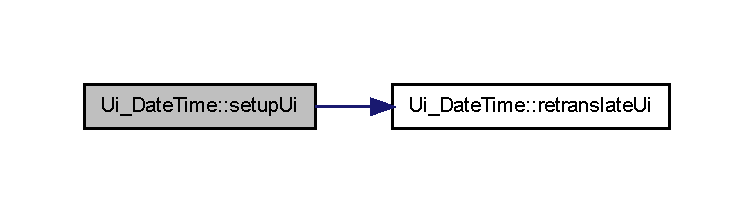
\includegraphics[width=362pt]{class_ui___date_time_aec460e980f671b301914cde3e3802143_cgraph}
\end{center}
\end{figure}




Here is the caller graph for this function:\nopagebreak
\begin{figure}[H]
\begin{center}
\leavevmode
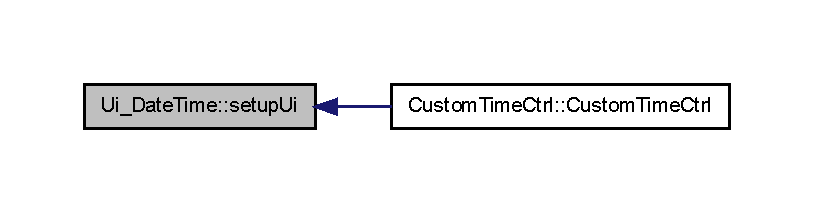
\includegraphics[width=390pt]{class_ui___date_time_aec460e980f671b301914cde3e3802143_icgraph}
\end{center}
\end{figure}




\subsection{Member Data Documentation}
\hypertarget{class_ui___date_time_acd3af509eccfb3a359c9a76ea8dfa2d4}{
\index{Ui\_\-DateTime@{Ui\_\-DateTime}!checkTime@{checkTime}}
\index{checkTime@{checkTime}!Ui_DateTime@{Ui\_\-DateTime}}
\subsubsection[{checkTime}]{\setlength{\rightskip}{0pt plus 5cm}QCheckBox$\ast$ {\bf Ui\_\-DateTime::checkTime}}}
\label{class_ui___date_time_acd3af509eccfb3a359c9a76ea8dfa2d4}
\hypertarget{class_ui___date_time_ac05a6b58da81b4d73730ab4deffc37d7}{
\index{Ui\_\-DateTime@{Ui\_\-DateTime}!dateEdit@{dateEdit}}
\index{dateEdit@{dateEdit}!Ui_DateTime@{Ui\_\-DateTime}}
\subsubsection[{dateEdit}]{\setlength{\rightskip}{0pt plus 5cm}QDateEdit$\ast$ {\bf Ui\_\-DateTime::dateEdit}}}
\label{class_ui___date_time_ac05a6b58da81b4d73730ab4deffc37d7}
\hypertarget{class_ui___date_time_afd7d89b895d622f67653fc453dc781a7}{
\index{Ui\_\-DateTime@{Ui\_\-DateTime}!gridLayout@{gridLayout}}
\index{gridLayout@{gridLayout}!Ui_DateTime@{Ui\_\-DateTime}}
\subsubsection[{gridLayout}]{\setlength{\rightskip}{0pt plus 5cm}QGridLayout$\ast$ {\bf Ui\_\-DateTime::gridLayout}}}
\label{class_ui___date_time_afd7d89b895d622f67653fc453dc781a7}
\hypertarget{class_ui___date_time_a5e283d401d2a14332b5c057dca4b5191}{
\index{Ui\_\-DateTime@{Ui\_\-DateTime}!gridLayout\_\-2@{gridLayout\_\-2}}
\index{gridLayout\_\-2@{gridLayout\_\-2}!Ui_DateTime@{Ui\_\-DateTime}}
\subsubsection[{gridLayout\_\-2}]{\setlength{\rightskip}{0pt plus 5cm}QGridLayout$\ast$ {\bf Ui\_\-DateTime::gridLayout\_\-2}}}
\label{class_ui___date_time_a5e283d401d2a14332b5c057dca4b5191}
\hypertarget{class_ui___date_time_aa589c9b11f049e55441921472edf5edb}{
\index{Ui\_\-DateTime@{Ui\_\-DateTime}!groupDate@{groupDate}}
\index{groupDate@{groupDate}!Ui_DateTime@{Ui\_\-DateTime}}
\subsubsection[{groupDate}]{\setlength{\rightskip}{0pt plus 5cm}QGroupBox$\ast$ {\bf Ui\_\-DateTime::groupDate}}}
\label{class_ui___date_time_aa589c9b11f049e55441921472edf5edb}
\hypertarget{class_ui___date_time_ae9887b3a8b4e56cf1cac0d542819c98d}{
\index{Ui\_\-DateTime@{Ui\_\-DateTime}!groupHasTime@{groupHasTime}}
\index{groupHasTime@{groupHasTime}!Ui_DateTime@{Ui\_\-DateTime}}
\subsubsection[{groupHasTime}]{\setlength{\rightskip}{0pt plus 5cm}QGroupBox$\ast$ {\bf Ui\_\-DateTime::groupHasTime}}}
\label{class_ui___date_time_ae9887b3a8b4e56cf1cac0d542819c98d}
\hypertarget{class_ui___date_time_a0228c72e4210b7e2325f003f7b0525bd}{
\index{Ui\_\-DateTime@{Ui\_\-DateTime}!groupTime@{groupTime}}
\index{groupTime@{groupTime}!Ui_DateTime@{Ui\_\-DateTime}}
\subsubsection[{groupTime}]{\setlength{\rightskip}{0pt plus 5cm}QGroupBox$\ast$ {\bf Ui\_\-DateTime::groupTime}}}
\label{class_ui___date_time_a0228c72e4210b7e2325f003f7b0525bd}
\hypertarget{class_ui___date_time_a2643fceafcdce6541af710a79f579301}{
\index{Ui\_\-DateTime@{Ui\_\-DateTime}!horizontalLayout@{horizontalLayout}}
\index{horizontalLayout@{horizontalLayout}!Ui_DateTime@{Ui\_\-DateTime}}
\subsubsection[{horizontalLayout}]{\setlength{\rightskip}{0pt plus 5cm}QHBoxLayout$\ast$ {\bf Ui\_\-DateTime::horizontalLayout}}}
\label{class_ui___date_time_a2643fceafcdce6541af710a79f579301}
\hypertarget{class_ui___date_time_a4a83e6da2cb4777c714707d0ec9ef071}{
\index{Ui\_\-DateTime@{Ui\_\-DateTime}!horizontalLayout\_\-2@{horizontalLayout\_\-2}}
\index{horizontalLayout\_\-2@{horizontalLayout\_\-2}!Ui_DateTime@{Ui\_\-DateTime}}
\subsubsection[{horizontalLayout\_\-2}]{\setlength{\rightskip}{0pt plus 5cm}QHBoxLayout$\ast$ {\bf Ui\_\-DateTime::horizontalLayout\_\-2}}}
\label{class_ui___date_time_a4a83e6da2cb4777c714707d0ec9ef071}
\hypertarget{class_ui___date_time_a2c9c40ac284a6523d361201e4c0c2ec7}{
\index{Ui\_\-DateTime@{Ui\_\-DateTime}!lbDate@{lbDate}}
\index{lbDate@{lbDate}!Ui_DateTime@{Ui\_\-DateTime}}
\subsubsection[{lbDate}]{\setlength{\rightskip}{0pt plus 5cm}QLabel$\ast$ {\bf Ui\_\-DateTime::lbDate}}}
\label{class_ui___date_time_a2c9c40ac284a6523d361201e4c0c2ec7}
\hypertarget{class_ui___date_time_ae2e82ce0d9b527827658c605e4f814e7}{
\index{Ui\_\-DateTime@{Ui\_\-DateTime}!lbDateFormat@{lbDateFormat}}
\index{lbDateFormat@{lbDateFormat}!Ui_DateTime@{Ui\_\-DateTime}}
\subsubsection[{lbDateFormat}]{\setlength{\rightskip}{0pt plus 5cm}QLabel$\ast$ {\bf Ui\_\-DateTime::lbDateFormat}}}
\label{class_ui___date_time_ae2e82ce0d9b527827658c605e4f814e7}
\hypertarget{class_ui___date_time_a3a3c6501192cd0e3d6586310689bcd3f}{
\index{Ui\_\-DateTime@{Ui\_\-DateTime}!lbTime@{lbTime}}
\index{lbTime@{lbTime}!Ui_DateTime@{Ui\_\-DateTime}}
\subsubsection[{lbTime}]{\setlength{\rightskip}{0pt plus 5cm}QLabel$\ast$ {\bf Ui\_\-DateTime::lbTime}}}
\label{class_ui___date_time_a3a3c6501192cd0e3d6586310689bcd3f}
\hypertarget{class_ui___date_time_a8701c245df77db5561ea1c0964c20a8f}{
\index{Ui\_\-DateTime@{Ui\_\-DateTime}!lbTimeFormat@{lbTimeFormat}}
\index{lbTimeFormat@{lbTimeFormat}!Ui_DateTime@{Ui\_\-DateTime}}
\subsubsection[{lbTimeFormat}]{\setlength{\rightskip}{0pt plus 5cm}QLabel$\ast$ {\bf Ui\_\-DateTime::lbTimeFormat}}}
\label{class_ui___date_time_a8701c245df77db5561ea1c0964c20a8f}
\hypertarget{class_ui___date_time_a37289c6e591cee258708a9736b503415}{
\index{Ui\_\-DateTime@{Ui\_\-DateTime}!timeEdit@{timeEdit}}
\index{timeEdit@{timeEdit}!Ui_DateTime@{Ui\_\-DateTime}}
\subsubsection[{timeEdit}]{\setlength{\rightskip}{0pt plus 5cm}QTimeEdit$\ast$ {\bf Ui\_\-DateTime::timeEdit}}}
\label{class_ui___date_time_a37289c6e591cee258708a9736b503415}
\hypertarget{class_ui___date_time_a5b1cbbfbf53e56fae7a1d7010cd6dd78}{
\index{Ui\_\-DateTime@{Ui\_\-DateTime}!verticalLayout@{verticalLayout}}
\index{verticalLayout@{verticalLayout}!Ui_DateTime@{Ui\_\-DateTime}}
\subsubsection[{verticalLayout}]{\setlength{\rightskip}{0pt plus 5cm}QVBoxLayout$\ast$ {\bf Ui\_\-DateTime::verticalLayout}}}
\label{class_ui___date_time_a5b1cbbfbf53e56fae7a1d7010cd6dd78}


The documentation for this class was generated from the following file:\begin{DoxyCompactItemize}
\item 
CustomTimeCtrl/GeneratedFiles/\hyperlink{ui__datetime_8h}{ui\_\-datetime.h}\end{DoxyCompactItemize}

\chapter{File Documentation}
\hypertarget{customtimectrl_8cpp}{
\section{CustomTimeCtrl/customtimectrl.cpp File Reference}
\label{customtimectrl_8cpp}\index{CustomTimeCtrl/customtimectrl.cpp@{CustomTimeCtrl/customtimectrl.cpp}}
}
{\ttfamily \#include \char`\"{}customtimectrl.h\char`\"{}}\par
Include dependency graph for customtimectrl.cpp:\nopagebreak
\begin{figure}[H]
\begin{center}
\leavevmode
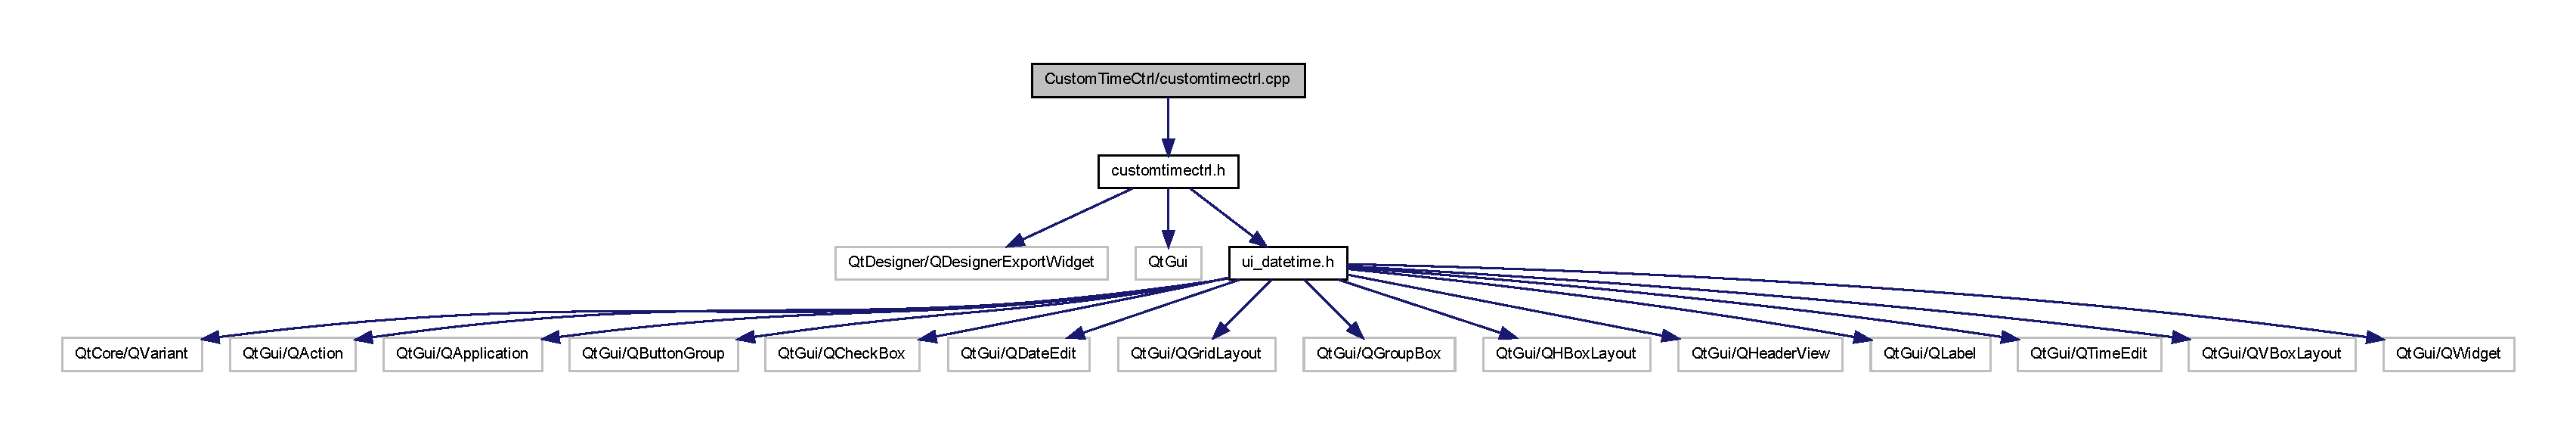
\includegraphics[width=400pt]{customtimectrl_8cpp__incl}
\end{center}
\end{figure}

\hypertarget{customtimectrl_8h}{
\section{CustomTimeCtrl/customtimectrl.h File Reference}
\label{customtimectrl_8h}\index{CustomTimeCtrl/customtimectrl.h@{CustomTimeCtrl/customtimectrl.h}}
}
{\ttfamily \#include $<$QtDesigner/QDesignerExportWidget$>$}\par
{\ttfamily \#include $<$QtGui$>$}\par
{\ttfamily \#include \char`\"{}ui\_\-datetime.h\char`\"{}}\par
Include dependency graph for customtimectrl.h:\nopagebreak
\begin{figure}[H]
\begin{center}
\leavevmode
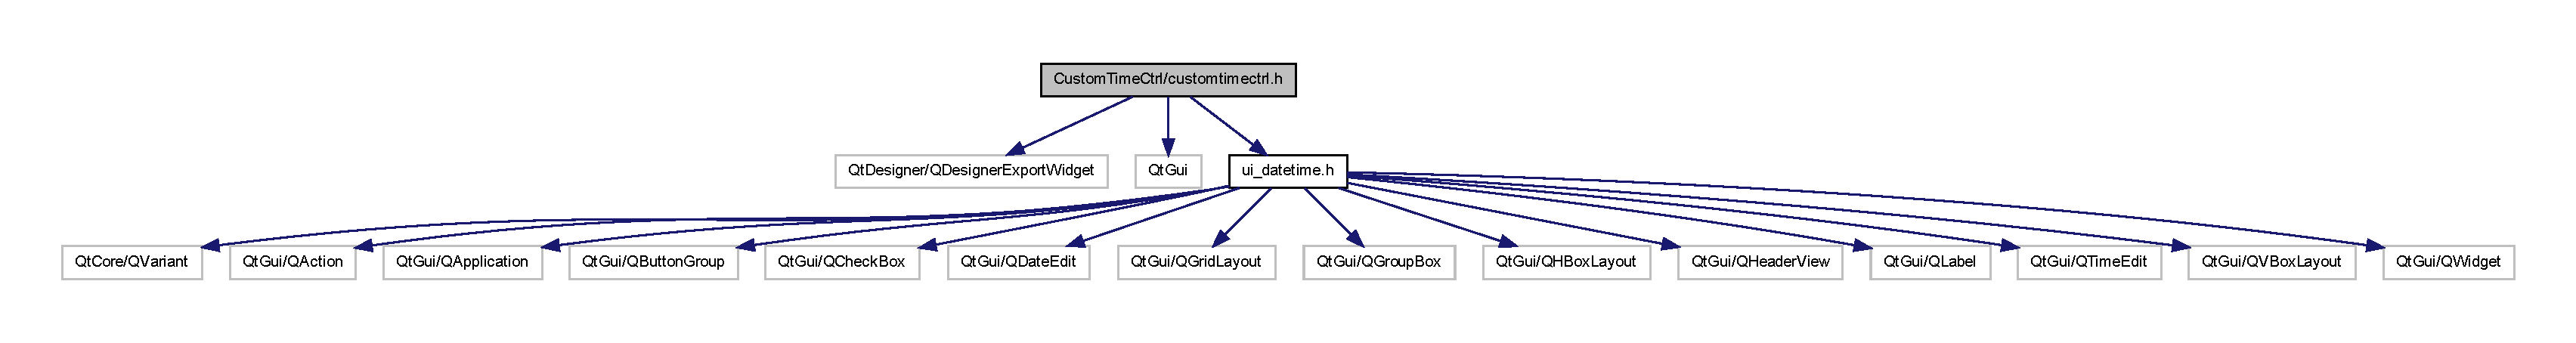
\includegraphics[width=400pt]{customtimectrl_8h__incl}
\end{center}
\end{figure}
This graph shows which files directly or indirectly include this file:\nopagebreak
\begin{figure}[H]
\begin{center}
\leavevmode
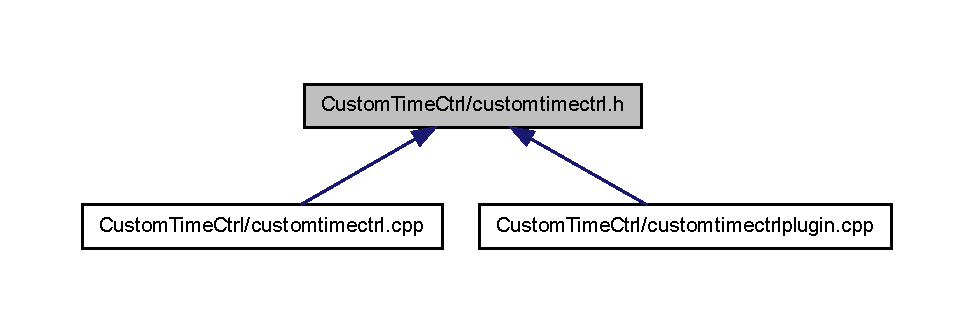
\includegraphics[width=400pt]{customtimectrl_8h__dep__incl}
\end{center}
\end{figure}
\subsection*{Classes}
\begin{DoxyCompactItemize}
\item 
class \hyperlink{class_custom_time_ctrl}{CustomTimeCtrl}
\begin{DoxyCompactList}\small\item\em Custom Time Control class. \item\end{DoxyCompactList}\end{DoxyCompactItemize}

\hypertarget{customtimectrlplugin_8cpp}{
\section{CustomTimeCtrl/customtimectrlplugin.cpp File Reference}
\label{customtimectrlplugin_8cpp}\index{CustomTimeCtrl/customtimectrlplugin.cpp@{CustomTimeCtrl/customtimectrlplugin.cpp}}
}
{\ttfamily \#include \char`\"{}customtimectrl.h\char`\"{}}\par
{\ttfamily \#include $<$QtCore/QtPlugin$>$}\par
{\ttfamily \#include \char`\"{}customtimectrlplugin.h\char`\"{}}\par
Include dependency graph for customtimectrlplugin.cpp:\nopagebreak
\begin{figure}[H]
\begin{center}
\leavevmode
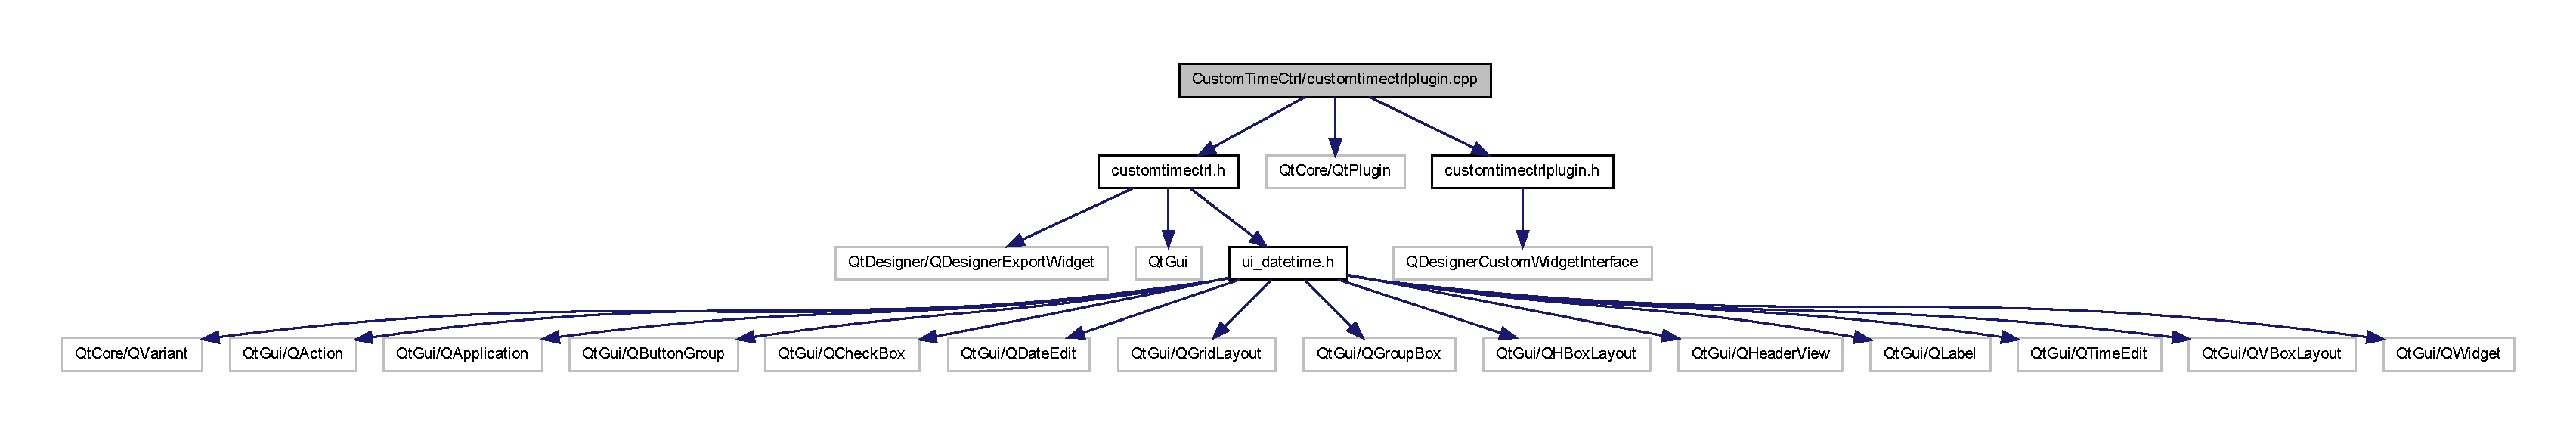
\includegraphics[width=400pt]{customtimectrlplugin_8cpp__incl}
\end{center}
\end{figure}

\hypertarget{customtimectrlplugin_8h}{
\section{CustomTimeCtrl/customtimectrlplugin.h File Reference}
\label{customtimectrlplugin_8h}\index{CustomTimeCtrl/customtimectrlplugin.h@{CustomTimeCtrl/customtimectrlplugin.h}}
}
{\ttfamily \#include $<$QDesignerCustomWidgetInterface$>$}\par
Include dependency graph for customtimectrlplugin.h:\nopagebreak
\begin{figure}[H]
\begin{center}
\leavevmode
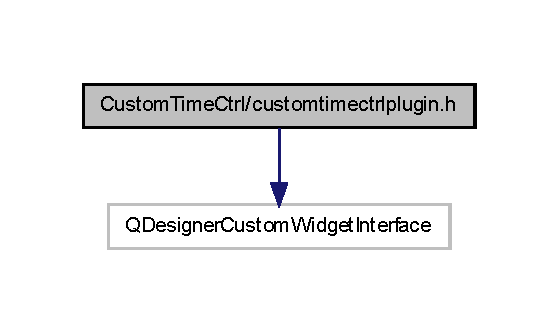
\includegraphics[width=268pt]{customtimectrlplugin_8h__incl}
\end{center}
\end{figure}
This graph shows which files directly or indirectly include this file:\nopagebreak
\begin{figure}[H]
\begin{center}
\leavevmode
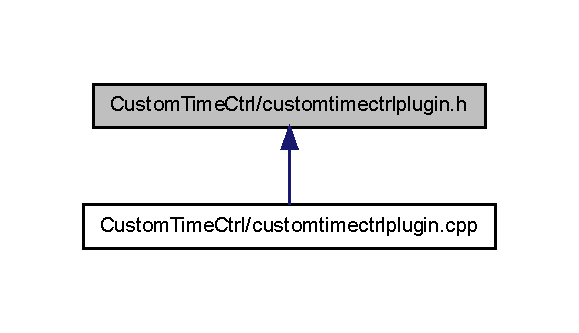
\includegraphics[width=278pt]{customtimectrlplugin_8h__dep__incl}
\end{center}
\end{figure}
\subsection*{Classes}
\begin{DoxyCompactItemize}
\item 
class \hyperlink{class_custom_time_ctrl_plugin}{CustomTimeCtrlPlugin}
\begin{DoxyCompactList}\small\item\em Plugin Class. \item\end{DoxyCompactList}\end{DoxyCompactItemize}

\hypertarget{_debug_2moc__customtimectrl_8cpp}{
\section{CustomTimeCtrl/GeneratedFiles/Debug/moc\_\-customtimectrl.cpp File Reference}
\label{_debug_2moc__customtimectrl_8cpp}\index{CustomTimeCtrl/GeneratedFiles/Debug/moc\_\-customtimectrl.cpp@{CustomTimeCtrl/GeneratedFiles/Debug/moc\_\-customtimectrl.cpp}}
}
{\ttfamily \#include \char`\"{}../../customtimectrl.h\char`\"{}}\par
Include dependency graph for moc\_\-customtimectrl.cpp:\nopagebreak
\begin{figure}[H]
\begin{center}
\leavevmode
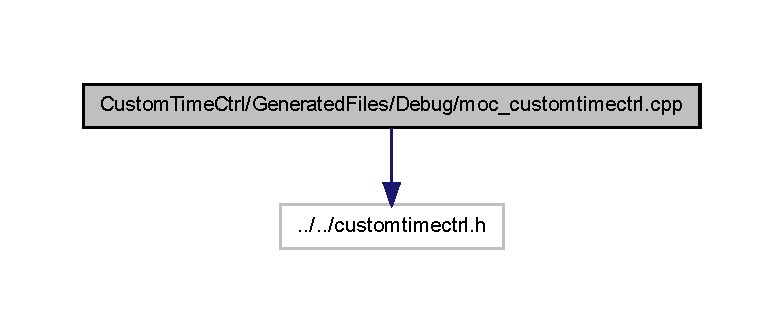
\includegraphics[width=376pt]{_debug_2moc__customtimectrl_8cpp__incl}
\end{center}
\end{figure}
\subsection*{Variables}
\begin{DoxyCompactItemize}
\item 
static QT\_\-BEGIN\_\-MOC\_\-NAMESPACE const uint \hyperlink{_debug_2moc__customtimectrl_8cpp_ae331268d7f0724fded0c156d3087035f}{qt\_\-meta\_\-data\_\-CustomTimeCtrl} \mbox{[}$\,$\mbox{]}
\item 
static const char \hyperlink{_debug_2moc__customtimectrl_8cpp_a1dc02345427486093715f8798da2acdd}{qt\_\-meta\_\-stringdata\_\-CustomTimeCtrl} \mbox{[}$\,$\mbox{]}
\end{DoxyCompactItemize}


\subsection{Variable Documentation}
\hypertarget{_debug_2moc__customtimectrl_8cpp_ae331268d7f0724fded0c156d3087035f}{
\index{Debug/moc\_\-customtimectrl.cpp@{Debug/moc\_\-customtimectrl.cpp}!qt\_\-meta\_\-data\_\-CustomTimeCtrl@{qt\_\-meta\_\-data\_\-CustomTimeCtrl}}
\index{qt\_\-meta\_\-data\_\-CustomTimeCtrl@{qt\_\-meta\_\-data\_\-CustomTimeCtrl}!Debug/moc_customtimectrl.cpp@{Debug/moc\_\-customtimectrl.cpp}}
\subsubsection[{qt\_\-meta\_\-data\_\-CustomTimeCtrl}]{\setlength{\rightskip}{0pt plus 5cm}QT\_\-BEGIN\_\-MOC\_\-NAMESPACE const uint {\bf qt\_\-meta\_\-data\_\-CustomTimeCtrl}\mbox{[}$\,$\mbox{]}\hspace{0.3cm}{\ttfamily  \mbox{[}static\mbox{]}}}}
\label{_debug_2moc__customtimectrl_8cpp_ae331268d7f0724fded0c156d3087035f}
{\bfseries Initial value:}
\begin{DoxyCode}
 {

 
       5,       
       0,       
       0,    0, 
       4,   14, 
       1,   34, 
       0,    0, 
       0,    0, 
       0,       
       2,       

 
      22,   16,   15,   15, 0x05,
      49,   35,   15,   15, 0x05,

 
      80,   70,   15,   15, 0x0a,
     123,  117,   15,   15, 0x08,

 
     150,  140, 0x10195103,

 
       0,

       0        
}
\end{DoxyCode}
\hypertarget{_debug_2moc__customtimectrl_8cpp_a1dc02345427486093715f8798da2acdd}{
\index{Debug/moc\_\-customtimectrl.cpp@{Debug/moc\_\-customtimectrl.cpp}!qt\_\-meta\_\-stringdata\_\-CustomTimeCtrl@{qt\_\-meta\_\-stringdata\_\-CustomTimeCtrl}}
\index{qt\_\-meta\_\-stringdata\_\-CustomTimeCtrl@{qt\_\-meta\_\-stringdata\_\-CustomTimeCtrl}!Debug/moc_customtimectrl.cpp@{Debug/moc\_\-customtimectrl.cpp}}
\subsubsection[{qt\_\-meta\_\-stringdata\_\-CustomTimeCtrl}]{\setlength{\rightskip}{0pt plus 5cm}const char {\bf qt\_\-meta\_\-stringdata\_\-CustomTimeCtrl}\mbox{[}$\,$\mbox{]}\hspace{0.3cm}{\ttfamily  \mbox{[}static\mbox{]}}}}
\label{_debug_2moc__customtimectrl_8cpp_a1dc02345427486093715f8798da2acdd}
{\bfseries Initial value:}
\begin{DoxyCode}
 {
    "CustomTimeCtrl\0\0bAuto\0isAuto(bool)\0"
    "bDateTime,row\0isDateTime(bool,int)\0"
    "index,var\0adjustDateTime(QModelIndex,QVariant)\0"
    "bTime\0setHasTime(bool)\0QDateTime\0"
    "dateTime\0"
}
\end{DoxyCode}

\hypertarget{_release_2moc__customtimectrl_8cpp}{
\section{CustomTimeCtrl/GeneratedFiles/Release/moc\_\-customtimectrl.cpp File Reference}
\label{_release_2moc__customtimectrl_8cpp}\index{CustomTimeCtrl/GeneratedFiles/Release/moc\_\-customtimectrl.cpp@{CustomTimeCtrl/GeneratedFiles/Release/moc\_\-customtimectrl.cpp}}
}
{\ttfamily \#include \char`\"{}../../customtimectrl.h\char`\"{}}\par
Include dependency graph for moc\_\-customtimectrl.cpp:\nopagebreak
\begin{figure}[H]
\begin{center}
\leavevmode
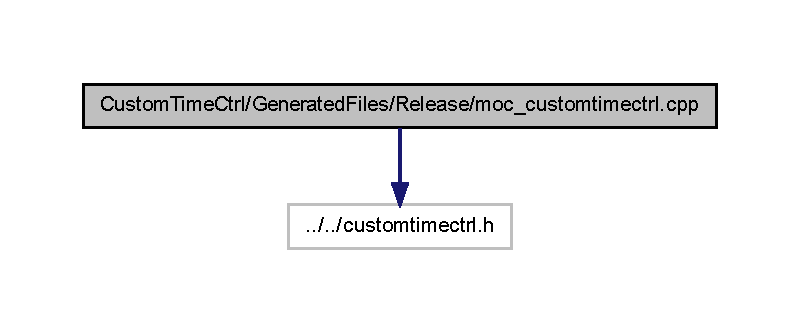
\includegraphics[width=384pt]{_release_2moc__customtimectrl_8cpp__incl}
\end{center}
\end{figure}
\subsection*{Variables}
\begin{DoxyCompactItemize}
\item 
static QT\_\-BEGIN\_\-MOC\_\-NAMESPACE const uint \hyperlink{_release_2moc__customtimectrl_8cpp_ae331268d7f0724fded0c156d3087035f}{qt\_\-meta\_\-data\_\-CustomTimeCtrl} \mbox{[}$\,$\mbox{]}
\item 
static const char \hyperlink{_release_2moc__customtimectrl_8cpp_a1dc02345427486093715f8798da2acdd}{qt\_\-meta\_\-stringdata\_\-CustomTimeCtrl} \mbox{[}$\,$\mbox{]}
\end{DoxyCompactItemize}


\subsection{Variable Documentation}
\hypertarget{_release_2moc__customtimectrl_8cpp_ae331268d7f0724fded0c156d3087035f}{
\index{Release/moc\_\-customtimectrl.cpp@{Release/moc\_\-customtimectrl.cpp}!qt\_\-meta\_\-data\_\-CustomTimeCtrl@{qt\_\-meta\_\-data\_\-CustomTimeCtrl}}
\index{qt\_\-meta\_\-data\_\-CustomTimeCtrl@{qt\_\-meta\_\-data\_\-CustomTimeCtrl}!Release/moc_customtimectrl.cpp@{Release/moc\_\-customtimectrl.cpp}}
\subsubsection[{qt\_\-meta\_\-data\_\-CustomTimeCtrl}]{\setlength{\rightskip}{0pt plus 5cm}QT\_\-BEGIN\_\-MOC\_\-NAMESPACE const uint {\bf qt\_\-meta\_\-data\_\-CustomTimeCtrl}\mbox{[}$\,$\mbox{]}\hspace{0.3cm}{\ttfamily  \mbox{[}static\mbox{]}}}}
\label{_release_2moc__customtimectrl_8cpp_ae331268d7f0724fded0c156d3087035f}
{\bfseries Initial value:}
\begin{DoxyCode}
 {

 
       5,       
       0,       
       0,    0, 
       4,   14, 
       1,   34, 
       0,    0, 
       0,    0, 
       0,       
       2,       

 
      22,   16,   15,   15, 0x05,
      49,   35,   15,   15, 0x05,

 
      80,   70,   15,   15, 0x0a,
     123,  117,   15,   15, 0x08,

 
     150,  140, 0x10195103,

 
       0,

       0        
}
\end{DoxyCode}
\hypertarget{_release_2moc__customtimectrl_8cpp_a1dc02345427486093715f8798da2acdd}{
\index{Release/moc\_\-customtimectrl.cpp@{Release/moc\_\-customtimectrl.cpp}!qt\_\-meta\_\-stringdata\_\-CustomTimeCtrl@{qt\_\-meta\_\-stringdata\_\-CustomTimeCtrl}}
\index{qt\_\-meta\_\-stringdata\_\-CustomTimeCtrl@{qt\_\-meta\_\-stringdata\_\-CustomTimeCtrl}!Release/moc_customtimectrl.cpp@{Release/moc\_\-customtimectrl.cpp}}
\subsubsection[{qt\_\-meta\_\-stringdata\_\-CustomTimeCtrl}]{\setlength{\rightskip}{0pt plus 5cm}const char {\bf qt\_\-meta\_\-stringdata\_\-CustomTimeCtrl}\mbox{[}$\,$\mbox{]}\hspace{0.3cm}{\ttfamily  \mbox{[}static\mbox{]}}}}
\label{_release_2moc__customtimectrl_8cpp_a1dc02345427486093715f8798da2acdd}
{\bfseries Initial value:}
\begin{DoxyCode}
 {
    "CustomTimeCtrl\0\0bAuto\0isAuto(bool)\0"
    "bDateTime,row\0isDateTime(bool,int)\0"
    "index,var\0adjustDateTime(QModelIndex,QVariant)\0"
    "bTime\0setHasTime(bool)\0QDateTime\0"
    "dateTime\0"
}
\end{DoxyCode}

\hypertarget{_debug_2moc__customtimectrlplugin_8cpp}{
\section{CustomTimeCtrl/GeneratedFiles/Debug/moc\_\-customtimectrlplugin.cpp File Reference}
\label{_debug_2moc__customtimectrlplugin_8cpp}\index{CustomTimeCtrl/GeneratedFiles/Debug/moc\_\-customtimectrlplugin.cpp@{CustomTimeCtrl/GeneratedFiles/Debug/moc\_\-customtimectrlplugin.cpp}}
}
{\ttfamily \#include \char`\"{}../../customtimectrlplugin.h\char`\"{}}\par
Include dependency graph for moc\_\-customtimectrlplugin.cpp:\nopagebreak
\begin{figure}[H]
\begin{center}
\leavevmode
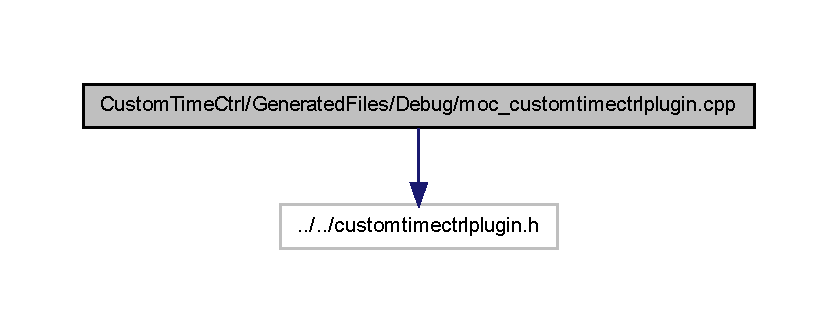
\includegraphics[width=400pt]{_debug_2moc__customtimectrlplugin_8cpp__incl}
\end{center}
\end{figure}
\subsection*{Variables}
\begin{DoxyCompactItemize}
\item 
static QT\_\-BEGIN\_\-MOC\_\-NAMESPACE const uint \hyperlink{_debug_2moc__customtimectrlplugin_8cpp_a66fa7762093948a240a610c6e57e9fcb}{qt\_\-meta\_\-data\_\-CustomTimeCtrlPlugin} \mbox{[}$\,$\mbox{]}
\item 
static const char \hyperlink{_debug_2moc__customtimectrlplugin_8cpp_af90f1acfbd089e2af56ea8d22d8ca4f0}{qt\_\-meta\_\-stringdata\_\-CustomTimeCtrlPlugin} \mbox{[}$\,$\mbox{]}
\end{DoxyCompactItemize}


\subsection{Variable Documentation}
\hypertarget{_debug_2moc__customtimectrlplugin_8cpp_a66fa7762093948a240a610c6e57e9fcb}{
\index{Debug/moc\_\-customtimectrlplugin.cpp@{Debug/moc\_\-customtimectrlplugin.cpp}!qt\_\-meta\_\-data\_\-CustomTimeCtrlPlugin@{qt\_\-meta\_\-data\_\-CustomTimeCtrlPlugin}}
\index{qt\_\-meta\_\-data\_\-CustomTimeCtrlPlugin@{qt\_\-meta\_\-data\_\-CustomTimeCtrlPlugin}!Debug/moc_customtimectrlplugin.cpp@{Debug/moc\_\-customtimectrlplugin.cpp}}
\subsubsection[{qt\_\-meta\_\-data\_\-CustomTimeCtrlPlugin}]{\setlength{\rightskip}{0pt plus 5cm}QT\_\-BEGIN\_\-MOC\_\-NAMESPACE const uint {\bf qt\_\-meta\_\-data\_\-CustomTimeCtrlPlugin}\mbox{[}$\,$\mbox{]}\hspace{0.3cm}{\ttfamily  \mbox{[}static\mbox{]}}}}
\label{_debug_2moc__customtimectrlplugin_8cpp_a66fa7762093948a240a610c6e57e9fcb}
{\bfseries Initial value:}
\begin{DoxyCode}
 {

 
       5,       
       0,       
       0,    0, 
       0,    0, 
       0,    0, 
       0,    0, 
       0,    0, 
       0,       
       0,       

       0        
}
\end{DoxyCode}
\hypertarget{_debug_2moc__customtimectrlplugin_8cpp_af90f1acfbd089e2af56ea8d22d8ca4f0}{
\index{Debug/moc\_\-customtimectrlplugin.cpp@{Debug/moc\_\-customtimectrlplugin.cpp}!qt\_\-meta\_\-stringdata\_\-CustomTimeCtrlPlugin@{qt\_\-meta\_\-stringdata\_\-CustomTimeCtrlPlugin}}
\index{qt\_\-meta\_\-stringdata\_\-CustomTimeCtrlPlugin@{qt\_\-meta\_\-stringdata\_\-CustomTimeCtrlPlugin}!Debug/moc_customtimectrlplugin.cpp@{Debug/moc\_\-customtimectrlplugin.cpp}}
\subsubsection[{qt\_\-meta\_\-stringdata\_\-CustomTimeCtrlPlugin}]{\setlength{\rightskip}{0pt plus 5cm}const char {\bf qt\_\-meta\_\-stringdata\_\-CustomTimeCtrlPlugin}\mbox{[}$\,$\mbox{]}\hspace{0.3cm}{\ttfamily  \mbox{[}static\mbox{]}}}}
\label{_debug_2moc__customtimectrlplugin_8cpp_af90f1acfbd089e2af56ea8d22d8ca4f0}
{\bfseries Initial value:}
\begin{DoxyCode}
 {
    "CustomTimeCtrlPlugin\0"
}
\end{DoxyCode}

\hypertarget{_release_2moc__customtimectrlplugin_8cpp}{
\section{CustomTimeCtrl/GeneratedFiles/Release/moc\_\-customtimectrlplugin.cpp File Reference}
\label{_release_2moc__customtimectrlplugin_8cpp}\index{CustomTimeCtrl/GeneratedFiles/Release/moc\_\-customtimectrlplugin.cpp@{CustomTimeCtrl/GeneratedFiles/Release/moc\_\-customtimectrlplugin.cpp}}
}
{\ttfamily \#include \char`\"{}../../customtimectrlplugin.h\char`\"{}}\par
Include dependency graph for moc\_\-customtimectrlplugin.cpp:\nopagebreak
\begin{figure}[H]
\begin{center}
\leavevmode
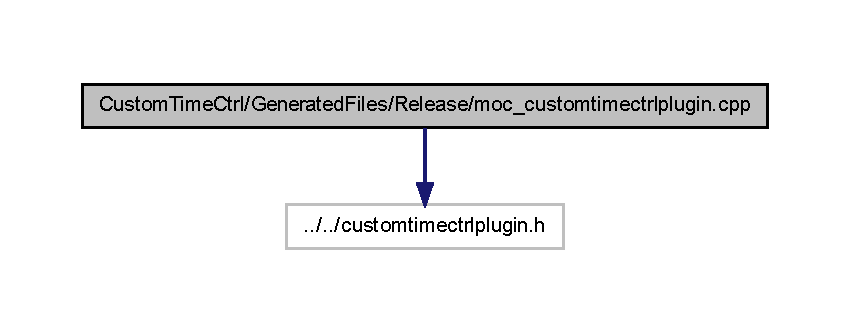
\includegraphics[width=400pt]{_release_2moc__customtimectrlplugin_8cpp__incl}
\end{center}
\end{figure}
\subsection*{Variables}
\begin{DoxyCompactItemize}
\item 
static QT\_\-BEGIN\_\-MOC\_\-NAMESPACE const uint \hyperlink{_release_2moc__customtimectrlplugin_8cpp_a66fa7762093948a240a610c6e57e9fcb}{qt\_\-meta\_\-data\_\-CustomTimeCtrlPlugin} \mbox{[}$\,$\mbox{]}
\item 
static const char \hyperlink{_release_2moc__customtimectrlplugin_8cpp_af90f1acfbd089e2af56ea8d22d8ca4f0}{qt\_\-meta\_\-stringdata\_\-CustomTimeCtrlPlugin} \mbox{[}$\,$\mbox{]}
\end{DoxyCompactItemize}


\subsection{Variable Documentation}
\hypertarget{_release_2moc__customtimectrlplugin_8cpp_a66fa7762093948a240a610c6e57e9fcb}{
\index{Release/moc\_\-customtimectrlplugin.cpp@{Release/moc\_\-customtimectrlplugin.cpp}!qt\_\-meta\_\-data\_\-CustomTimeCtrlPlugin@{qt\_\-meta\_\-data\_\-CustomTimeCtrlPlugin}}
\index{qt\_\-meta\_\-data\_\-CustomTimeCtrlPlugin@{qt\_\-meta\_\-data\_\-CustomTimeCtrlPlugin}!Release/moc_customtimectrlplugin.cpp@{Release/moc\_\-customtimectrlplugin.cpp}}
\subsubsection[{qt\_\-meta\_\-data\_\-CustomTimeCtrlPlugin}]{\setlength{\rightskip}{0pt plus 5cm}QT\_\-BEGIN\_\-MOC\_\-NAMESPACE const uint {\bf qt\_\-meta\_\-data\_\-CustomTimeCtrlPlugin}\mbox{[}$\,$\mbox{]}\hspace{0.3cm}{\ttfamily  \mbox{[}static\mbox{]}}}}
\label{_release_2moc__customtimectrlplugin_8cpp_a66fa7762093948a240a610c6e57e9fcb}
{\bfseries Initial value:}
\begin{DoxyCode}
 {

 
       5,       
       0,       
       0,    0, 
       0,    0, 
       0,    0, 
       0,    0, 
       0,    0, 
       0,       
       0,       

       0        
}
\end{DoxyCode}
\hypertarget{_release_2moc__customtimectrlplugin_8cpp_af90f1acfbd089e2af56ea8d22d8ca4f0}{
\index{Release/moc\_\-customtimectrlplugin.cpp@{Release/moc\_\-customtimectrlplugin.cpp}!qt\_\-meta\_\-stringdata\_\-CustomTimeCtrlPlugin@{qt\_\-meta\_\-stringdata\_\-CustomTimeCtrlPlugin}}
\index{qt\_\-meta\_\-stringdata\_\-CustomTimeCtrlPlugin@{qt\_\-meta\_\-stringdata\_\-CustomTimeCtrlPlugin}!Release/moc_customtimectrlplugin.cpp@{Release/moc\_\-customtimectrlplugin.cpp}}
\subsubsection[{qt\_\-meta\_\-stringdata\_\-CustomTimeCtrlPlugin}]{\setlength{\rightskip}{0pt plus 5cm}const char {\bf qt\_\-meta\_\-stringdata\_\-CustomTimeCtrlPlugin}\mbox{[}$\,$\mbox{]}\hspace{0.3cm}{\ttfamily  \mbox{[}static\mbox{]}}}}
\label{_release_2moc__customtimectrlplugin_8cpp_af90f1acfbd089e2af56ea8d22d8ca4f0}
{\bfseries Initial value:}
\begin{DoxyCode}
 {
    "CustomTimeCtrlPlugin\0"
}
\end{DoxyCode}

\hypertarget{qrc__customtimectrl_8cpp}{
\section{CustomTimeCtrl/GeneratedFiles/qrc\_\-customtimectrl.cpp File Reference}
\label{qrc__customtimectrl_8cpp}\index{CustomTimeCtrl/GeneratedFiles/qrc\_\-customtimectrl.cpp@{CustomTimeCtrl/GeneratedFiles/qrc\_\-customtimectrl.cpp}}
}
{\ttfamily \#include $<$QtCore/qglobal.h$>$}\par
Include dependency graph for qrc\_\-customtimectrl.cpp:\nopagebreak
\begin{figure}[H]
\begin{center}
\leavevmode
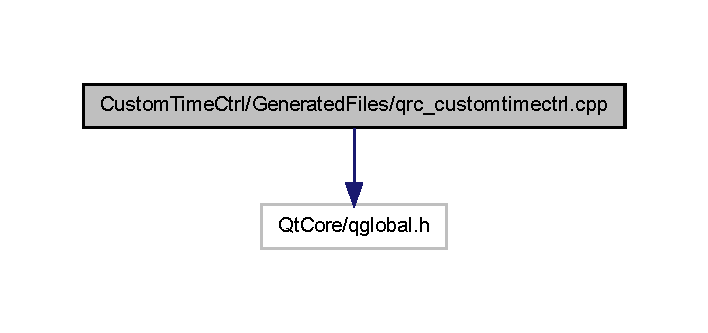
\includegraphics[width=340pt]{qrc__customtimectrl_8cpp__incl}
\end{center}
\end{figure}
\subsection*{Functions}
\begin{DoxyCompactItemize}
\item 
QT\_\-BEGIN\_\-NAMESPACE Q\_\-CORE\_\-EXPORT bool \hyperlink{qrc__customtimectrl_8cpp_ab3bec3d1e679084be46edc41e4c91bc1}{qRegisterResourceData} (int, const unsigned char $\ast$, const unsigned char $\ast$, const unsigned char $\ast$)
\item 
Q\_\-CORE\_\-EXPORT bool \hyperlink{qrc__customtimectrl_8cpp_ad65f8bca8010dd1fd135a28a085c6d03}{qUnregisterResourceData} (int, const unsigned char $\ast$, const unsigned char $\ast$, const unsigned char $\ast$)
\item 
QT\_\-END\_\-NAMESPACE int QT\_\-MANGLE\_\-NAMESPACE() \hyperlink{qrc__customtimectrl_8cpp_a63bc351592b10ff80737d1f1a558c038}{qInitResources\_\-customtimectrl} ()
\item 
int QT\_\-MANGLE\_\-NAMESPACE() \hyperlink{qrc__customtimectrl_8cpp_a646f8bacdf20fa77d99ac0615d7d207f}{qCleanupResources\_\-customtimectrl} ()
\end{DoxyCompactItemize}
\subsection*{Variables}
\begin{DoxyCompactItemize}
\item 
static const unsigned char \hyperlink{qrc__customtimectrl_8cpp_a67a985282ed24629b630f624b668842b}{qt\_\-resource\_\-data} \mbox{[}$\,$\mbox{]}
\item 
static const unsigned char \hyperlink{qrc__customtimectrl_8cpp_a7931167bf9d7e883e4194a60d031e431}{qt\_\-resource\_\-name} \mbox{[}$\,$\mbox{]}
\item 
static const unsigned char \hyperlink{qrc__customtimectrl_8cpp_a37a83d7da2ee18badcd100d79aac64d4}{qt\_\-resource\_\-struct} \mbox{[}$\,$\mbox{]}
\end{DoxyCompactItemize}


\subsection{Function Documentation}
\hypertarget{qrc__customtimectrl_8cpp_a646f8bacdf20fa77d99ac0615d7d207f}{
\index{qrc\_\-customtimectrl.cpp@{qrc\_\-customtimectrl.cpp}!qCleanupResources\_\-customtimectrl@{qCleanupResources\_\-customtimectrl}}
\index{qCleanupResources\_\-customtimectrl@{qCleanupResources\_\-customtimectrl}!qrc_customtimectrl.cpp@{qrc\_\-customtimectrl.cpp}}
\subsubsection[{qCleanupResources\_\-customtimectrl}]{\setlength{\rightskip}{0pt plus 5cm}int QT\_\-MANGLE\_\-NAMESPACE() qCleanupResources\_\-customtimectrl (
\begin{DoxyParamCaption}
{}
\end{DoxyParamCaption}
)}}
\label{qrc__customtimectrl_8cpp_a646f8bacdf20fa77d99ac0615d7d207f}


Here is the call graph for this function:\nopagebreak
\begin{figure}[H]
\begin{center}
\leavevmode
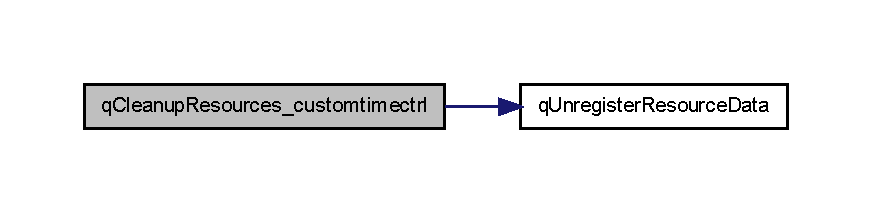
\includegraphics[width=400pt]{qrc__customtimectrl_8cpp_a646f8bacdf20fa77d99ac0615d7d207f_cgraph}
\end{center}
\end{figure}


\hypertarget{qrc__customtimectrl_8cpp_a63bc351592b10ff80737d1f1a558c038}{
\index{qrc\_\-customtimectrl.cpp@{qrc\_\-customtimectrl.cpp}!qInitResources\_\-customtimectrl@{qInitResources\_\-customtimectrl}}
\index{qInitResources\_\-customtimectrl@{qInitResources\_\-customtimectrl}!qrc_customtimectrl.cpp@{qrc\_\-customtimectrl.cpp}}
\subsubsection[{qInitResources\_\-customtimectrl}]{\setlength{\rightskip}{0pt plus 5cm}QT\_\-END\_\-NAMESPACE int QT\_\-MANGLE\_\-NAMESPACE() qInitResources\_\-customtimectrl (
\begin{DoxyParamCaption}
{}
\end{DoxyParamCaption}
)}}
\label{qrc__customtimectrl_8cpp_a63bc351592b10ff80737d1f1a558c038}


Here is the call graph for this function:\nopagebreak
\begin{figure}[H]
\begin{center}
\leavevmode
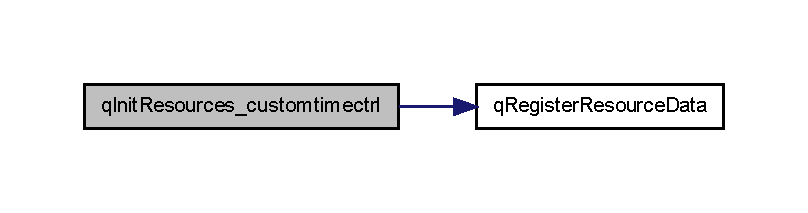
\includegraphics[width=388pt]{qrc__customtimectrl_8cpp_a63bc351592b10ff80737d1f1a558c038_cgraph}
\end{center}
\end{figure}


\hypertarget{qrc__customtimectrl_8cpp_ab3bec3d1e679084be46edc41e4c91bc1}{
\index{qrc\_\-customtimectrl.cpp@{qrc\_\-customtimectrl.cpp}!qRegisterResourceData@{qRegisterResourceData}}
\index{qRegisterResourceData@{qRegisterResourceData}!qrc_customtimectrl.cpp@{qrc\_\-customtimectrl.cpp}}
\subsubsection[{qRegisterResourceData}]{\setlength{\rightskip}{0pt plus 5cm}QT\_\-BEGIN\_\-NAMESPACE Q\_\-CORE\_\-EXPORT bool qRegisterResourceData (
\begin{DoxyParamCaption}
\item[{int}]{, }
\item[{const unsigned char $\ast$}]{, }
\item[{const unsigned char $\ast$}]{, }
\item[{const unsigned char $\ast$}]{}
\end{DoxyParamCaption}
)}}
\label{qrc__customtimectrl_8cpp_ab3bec3d1e679084be46edc41e4c91bc1}


Here is the caller graph for this function:\nopagebreak
\begin{figure}[H]
\begin{center}
\leavevmode
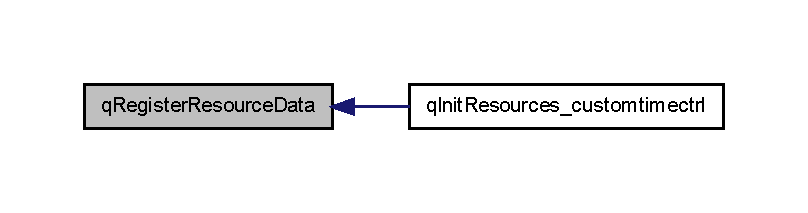
\includegraphics[width=388pt]{qrc__customtimectrl_8cpp_ab3bec3d1e679084be46edc41e4c91bc1_icgraph}
\end{center}
\end{figure}


\hypertarget{qrc__customtimectrl_8cpp_ad65f8bca8010dd1fd135a28a085c6d03}{
\index{qrc\_\-customtimectrl.cpp@{qrc\_\-customtimectrl.cpp}!qUnregisterResourceData@{qUnregisterResourceData}}
\index{qUnregisterResourceData@{qUnregisterResourceData}!qrc_customtimectrl.cpp@{qrc\_\-customtimectrl.cpp}}
\subsubsection[{qUnregisterResourceData}]{\setlength{\rightskip}{0pt plus 5cm}Q\_\-CORE\_\-EXPORT bool qUnregisterResourceData (
\begin{DoxyParamCaption}
\item[{int}]{, }
\item[{const unsigned char $\ast$}]{, }
\item[{const unsigned char $\ast$}]{, }
\item[{const unsigned char $\ast$}]{}
\end{DoxyParamCaption}
)}}
\label{qrc__customtimectrl_8cpp_ad65f8bca8010dd1fd135a28a085c6d03}


Here is the caller graph for this function:\nopagebreak
\begin{figure}[H]
\begin{center}
\leavevmode
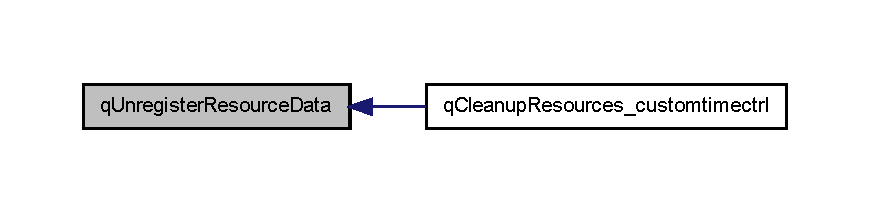
\includegraphics[width=400pt]{qrc__customtimectrl_8cpp_ad65f8bca8010dd1fd135a28a085c6d03_icgraph}
\end{center}
\end{figure}




\subsection{Variable Documentation}
\hypertarget{qrc__customtimectrl_8cpp_a67a985282ed24629b630f624b668842b}{
\index{qrc\_\-customtimectrl.cpp@{qrc\_\-customtimectrl.cpp}!qt\_\-resource\_\-data@{qt\_\-resource\_\-data}}
\index{qt\_\-resource\_\-data@{qt\_\-resource\_\-data}!qrc_customtimectrl.cpp@{qrc\_\-customtimectrl.cpp}}
\subsubsection[{qt\_\-resource\_\-data}]{\setlength{\rightskip}{0pt plus 5cm}const unsigned char {\bf qt\_\-resource\_\-data}\mbox{[}$\,$\mbox{]}\hspace{0.3cm}{\ttfamily  \mbox{[}static\mbox{]}}}}
\label{qrc__customtimectrl_8cpp_a67a985282ed24629b630f624b668842b}
\hypertarget{qrc__customtimectrl_8cpp_a7931167bf9d7e883e4194a60d031e431}{
\index{qrc\_\-customtimectrl.cpp@{qrc\_\-customtimectrl.cpp}!qt\_\-resource\_\-name@{qt\_\-resource\_\-name}}
\index{qt\_\-resource\_\-name@{qt\_\-resource\_\-name}!qrc_customtimectrl.cpp@{qrc\_\-customtimectrl.cpp}}
\subsubsection[{qt\_\-resource\_\-name}]{\setlength{\rightskip}{0pt plus 5cm}const unsigned char {\bf qt\_\-resource\_\-name}\mbox{[}$\,$\mbox{]}\hspace{0.3cm}{\ttfamily  \mbox{[}static\mbox{]}}}}
\label{qrc__customtimectrl_8cpp_a7931167bf9d7e883e4194a60d031e431}
{\bfseries Initial value:}
\begin{DoxyCode}
 {
  
  0x0,0xa,
  0x4,0xb0,0xac,0xc7,
  0x0,0x61,
  0x0,0x67,0x0,0x65,0x0,0x6e,0x0,0x64,0x0,0x61,0x0,0x2e,0x0,0x70,0x0,0x6e,0x0,0x6
      7,
  
}
\end{DoxyCode}
\hypertarget{qrc__customtimectrl_8cpp_a37a83d7da2ee18badcd100d79aac64d4}{
\index{qrc\_\-customtimectrl.cpp@{qrc\_\-customtimectrl.cpp}!qt\_\-resource\_\-struct@{qt\_\-resource\_\-struct}}
\index{qt\_\-resource\_\-struct@{qt\_\-resource\_\-struct}!qrc_customtimectrl.cpp@{qrc\_\-customtimectrl.cpp}}
\subsubsection[{qt\_\-resource\_\-struct}]{\setlength{\rightskip}{0pt plus 5cm}const unsigned char {\bf qt\_\-resource\_\-struct}\mbox{[}$\,$\mbox{]}\hspace{0.3cm}{\ttfamily  \mbox{[}static\mbox{]}}}}
\label{qrc__customtimectrl_8cpp_a37a83d7da2ee18badcd100d79aac64d4}
{\bfseries Initial value:}
\begin{DoxyCode}
 {
  
  0x0,0x0,0x0,0x0,0x0,0x2,0x0,0x0,0x0,0x1,0x0,0x0,0x0,0x1,
  
  0x0,0x0,0x0,0x0,0x0,0x0,0x0,0x0,0x0,0x1,0x0,0x0,0x0,0x0,

}
\end{DoxyCode}

\hypertarget{ui__datetime_8h}{
\section{CustomTimeCtrl/GeneratedFiles/ui\_\-datetime.h File Reference}
\label{ui__datetime_8h}\index{CustomTimeCtrl/GeneratedFiles/ui\_\-datetime.h@{CustomTimeCtrl/GeneratedFiles/ui\_\-datetime.h}}
}
{\ttfamily \#include $<$QtCore/QVariant$>$}\par
{\ttfamily \#include $<$QtGui/QAction$>$}\par
{\ttfamily \#include $<$QtGui/QApplication$>$}\par
{\ttfamily \#include $<$QtGui/QButtonGroup$>$}\par
{\ttfamily \#include $<$QtGui/QCheckBox$>$}\par
{\ttfamily \#include $<$QtGui/QDateEdit$>$}\par
{\ttfamily \#include $<$QtGui/QGridLayout$>$}\par
{\ttfamily \#include $<$QtGui/QGroupBox$>$}\par
{\ttfamily \#include $<$QtGui/QHBoxLayout$>$}\par
{\ttfamily \#include $<$QtGui/QHeaderView$>$}\par
{\ttfamily \#include $<$QtGui/QLabel$>$}\par
{\ttfamily \#include $<$QtGui/QTimeEdit$>$}\par
{\ttfamily \#include $<$QtGui/QVBoxLayout$>$}\par
{\ttfamily \#include $<$QtGui/QWidget$>$}\par
Include dependency graph for ui\_\-datetime.h:\nopagebreak
\begin{figure}[H]
\begin{center}
\leavevmode
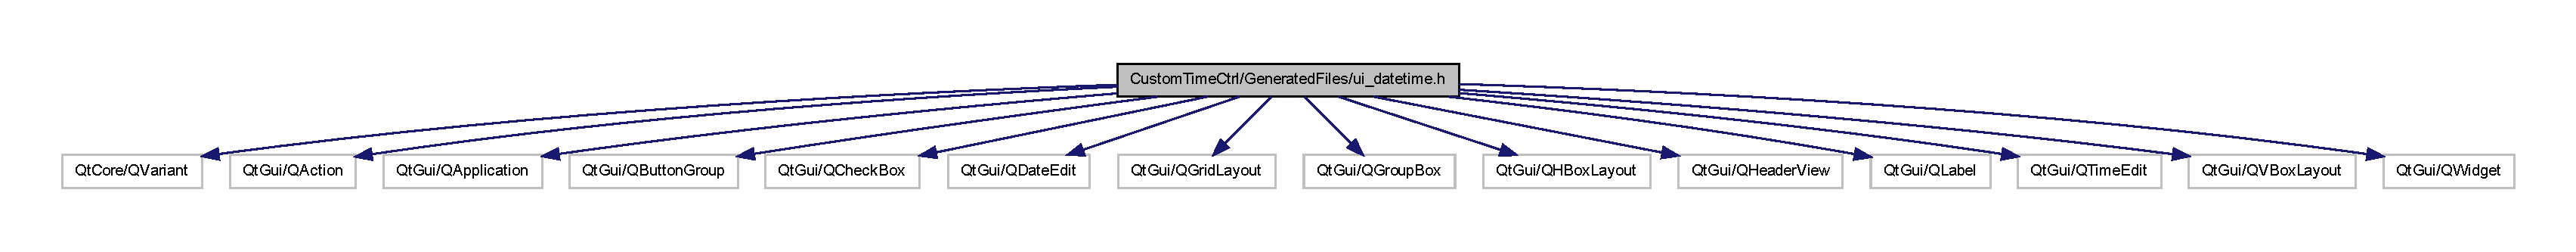
\includegraphics[width=400pt]{ui__datetime_8h__incl}
\end{center}
\end{figure}
This graph shows which files directly or indirectly include this file:\nopagebreak
\begin{figure}[H]
\begin{center}
\leavevmode
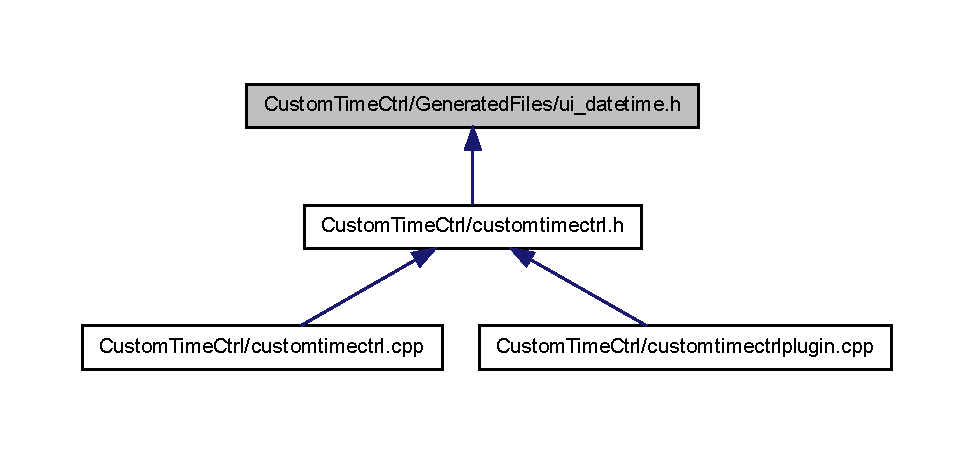
\includegraphics[width=400pt]{ui__datetime_8h__dep__incl}
\end{center}
\end{figure}
\subsection*{Classes}
\begin{DoxyCompactItemize}
\item 
class \hyperlink{class_ui___date_time}{Ui\_\-DateTime}
\item 
class \hyperlink{class_ui_1_1_date_time}{Ui::DateTime}
\end{DoxyCompactItemize}
\subsection*{Namespaces}
\begin{DoxyCompactItemize}
\item 
namespace \hyperlink{namespace_ui}{Ui}
\end{DoxyCompactItemize}

\printindex
\end{document}
